\documentclass[
version=last,toc=bib,toc=graduated,toc=index,toc=listof,9pt,openany]{scrbook}
%\pdfminorversion=4
\usepackage[utf8]{inputenc}
\usepackage[ngerman, english]{babel}
\usepackage{dejavu}

\usepackage{ifmtarg}
\usepackage{ifthen}

\usepackage{geometry}
\geometry{%a6paper
paperwidth=125mm, paperheight=168mm, 
portrait,
top=22mm, inner=22mm, outer=20mm, bottom=25mm,
headsep=3mm, footskip=12mm
}
\usepackage{lscape}
\setlength{\parskip}{0pt}

%\pdfminorversion=4


%\usepackage[babel,german=quotes]{csquotes}
\usepackage{relsize}

\clubpenalty=10000 %keine Schusterjungen
 \widowpenalty=10000 
 \displaywidowpenalty=10000 % keine Hurenkinder

\usepackage[letterspace=16]{microtype} %schönerer Textsatz

\usepackage{graphicx} %Bilder

%Dateipfade, wo die Bilder liegen
\graphicspath{{images-print/}{icons/}{extra-pages/}{wallpaper/}}
\usepackage{floatflt} % umflossene Logos
\usepackage{wrapfig}  % umflossene Logos von Sponsoren mit Multiabsatztexten

\usepackage{tabu}
\usepackage{tabularx}
\usepackage{longtable}
\usepackage[table,cymk]{xcolor}
\usepackage{colortbl}

% PDF-Seiten einbinden
% pdfpages, darf erst nach colortbl geladen werden!
\usepackage{pdfpages}

% PDFs als Hintergrundbilder
% wallpaper, darf erst nach colortbl geladen werden!
\usepackage{wallpaper}
\usepackage{multirow}
\usepackage{booktabs}
\usepackage{array}
\usepackage[manualmark]{scrpage2}
\pagestyle{scrplain}


\newcommand{\acro}[1]{{\textsmaller{#1}}} % Akronyme

% Überschriften in DejaVu Sans Condensed
\addtokomafont{sectioning}{\fontfamily{DejaVuSansCondensed-TLF}\selectfont}
\addtokomafont{pageheadfoot}{\usefont{T1}{DejaVuSansCondensed-TLF}{m}{n}}
\addtokomafont{pagenumber}{\usefont{T1}{DejaVuSansCondensed-TLF}{m}{n}}


%Titelei
\title{FOSSGIS 2015}
\subtitle{Programm}
\author{FOSSGIS e.V.}
\date{\today}

%\newcommand{\talkroom}{}
\clearscrheadings

% Seitenzahlen
\cfoot[\begin{small}\pagemark\end{small}]{\begin{small}\pagemark\end{small}}
\ofoot[]{}
\ifoot[]{}
\pagestyle{scrplain}

% Durchschuss erhöhen
\linespread{1.15}

% Befehlsdefinitionen einbinden
% neuer Zeitslot
\newcommand{\talktime}{9:99}
\newcommand{\newtimeslot}[1]{\newpage\renewcommand{\talktime}{#1}}

% neuer Zeitslot ohne Seitenumbruch
\newcommand{\newsmalltimeslot}[1]{\renewcommand{\talktime}{#1}}

% \konferenztag initialisieren
\newcommand{\konferenztag}{KeinTag}


% Hintergrund setzen
\def\mittwoch{Mittwoch}
\def\donnerstag{Donnerstag}
\def\freitag{Freitag}
\newcommand{\setpagebackground}{ %
%	\ifthispageodd{\ThisCenterWallPaper{1.0}{freitag-ungerade}}{\ThisCenterWallPaper{1.0}{freitag-gerade}}%
	\ifthenelse{\equal{\konferenztag}{\mittwoch}}{ %
		\ifthispageodd{\ThisCenterWallPaper{1.0}{mittwoch-ungerade}}{\ThisCenterWallPaper{1.0}{mittwoch-gerade}}%
	}{}
	\ifthenelse{\equal{\konferenztag}{\donnerstag}}{ %
		\ifthispageodd{\ThisCenterWallPaper{1.0}{donnerstag-ungerade}}{\ThisCenterWallPaper{1.0}{donnerstag-gerade}}%
	}{}
	\ifthenelse{\equal{\konferenztag}{\freitag}}{ %
		\ifthispageodd{\ThisCenterWallPaper{1.0}{freitag-ungerade}}{\ThisCenterWallPaper{1.0}{freitag-gerade}}%
	}{}
}


% Titeltabelle setzen
\newcolumntype{Y}[1]{>{\raggedright\arraybackslash}p{#1}}

\newcommand{\setabstract}[6]{
	% 1. Sprecher
	% 2. Titel
	% 3. Untertitel
	% 4. Abstract (Text)
	% 5. Farbe
	% 6. Raum
	\thispagestyle{scrheadings} 
	\setlength\tabcolsep{0pt}
	% \setlength{\fboxsep}{0pt}
	\noindent\colorbox{#5}{%
		\noindent\begin{tabu}{X[5L]r}
			\emph{#1} % Sprecher
			&
			\talktime
			\tabularnewline
			{\par\noindent\large \sectfont #2}% % Titel
			&
			#6
			\tabularnewline
			\issubtitleempty{#3}
%			\multicolumn{2}{p{\linewidth}}{\issubtitleempty{#3}}
%			\tabularnewline
		\end{tabu}%
	}
	%
	\isabstractempty{#4}%
	\setpagebackground%
	\vspace{0.5em}% Abstand zum nächsten Talk, auch wenn es keinen Abstract gibt
	\setlength\tabcolsep{6pt} % Spaltenpadding wieder auf Default setzen
}



% Setzen des Untertitels
% muss ausgelagert und durch \makeatletter umgeben sein
\makeatletter
\newcommand{\issubtitleempty}[1]{%
	\@ifnotmtarg{#1}{\multicolumn{2}{Y{\linewidth}}{\vspace{-0.6em} \noindent\bfseries \normalsize \sectfont #1}\tabularnewline}
}
\makeatother

% Setzen des Abstracts, falls vorhanden
% muss ausgelagert und durch \makeatletter umgeben sein
\makeatletter
\newcommand{\isabstractempty}[1]{%
		\vspace{0.5em}%
		\par\noindent #1 \par% % Abstract
		\vspace{1.5em}% Abstand zum nächsten Talk, auch wenn es einen Abstract gibt
}
\makeatother

% Farben definieren
\definecolor{eins}{cmyk}{ 0 .18 .06 .10}
\definecolor{zwei}{cmyk}{ .1 0 .17 .05}
\definecolor{zehn}{cmyk}{ 0 0.13 0.35 0.03}
\definecolor{aula}{cmyk}{ 0.2 0 0.05 0.13}

% Abstract Saal S10
\newcommand{\abstractZehn}[4]%
{%
	\setabstract{#1}{#2}{#3}{#4}{zehn}{S\,10}
}

% Abstract Saal S2
\newcommand{\abstractZwei}[4]%
{%
	\setabstract{#1}{#2}{#3}{#4}{zwei}{S\,2}
}

% Abstract Saal S1
\newcommand{\abstractEins}[4]%
{%
	\setabstract{#1}{#2}{#3}{#4}{eins}{S\,1}
}

% Abstract Aula
\newcommand{\abstractAula}[4]%
{%
	\setabstract{#1}{#2}{#3}{#4}{orange}{Aula}
}

% Abstract Senatssaal
%TODO Farbe ändern
\newcommand{\abstractSenatssaal}[4]%
{%
	\setabstract{#1}{#2}{#3}{#4}{orange}{Senatssaal}
}

% viel zu lang
\newcommand{\zulang}{Dieser Text ist viel zu lang. Dieser Text ist viel zu lang. Dieser Text ist viel zu lang. Dieser Text ist viel zu lang. Dieser Text ist viel zu lang. Dieser Text ist viel zu lang. Dieser Text ist viel zu lang. Dieser Text ist viel zu lang. Dieser Text ist viel zu lang. Dieser Text ist viel zu lang. Dieser Text ist viel zu lang. Dieser Text ist viel zu lang. Dieser Text ist viel zu lang. Dieser Text ist viel zu lang. }


\begin{document}
\lsstyle
\usefont{T1}{DejaVuSansCondensed-TLF}{m}{n}

% Schneidemarken
% Befehl zum Aufrufen definieren
\newcommand{\cropmarkswallpaper}{%
\CenterWallPaper{1.0}{crop-marks}%
}
\cropmarkswallpaper

\begin{titlepage}
\ClearWallPaper

\includepdf{deckseite-vektor-mit-schnittmarken}
\cropmarkswallpaper
\end{titlepage}

\section*{Inhaltsverzeichnis}


\vspace*{0.35em}%
\noindent Mittwoch \dotfill \pageref{mittwoch}

\vspace*{0.35em}%
\noindent Donnerstag \dotfill \pageref{donnerstag}

\vspace*{0.35em}%
\noindent Freitag \dotfill \pageref{freitag}

\vspace*{0.35em}%
\noindent Impressum \dotfill \pageref{impressum}\\

\newpage

\newpage
\newpage
\section*{Willkommen zur FOSSGIS-Konferenz 2014 in Münster!} \label{welcome}
Willkommen zur FOSSGIS-Konferenz 2014 in Münster!

FOSSGIS steht für Freie und Open Source Software für Geoinformationssysteme. 
Die FOSSGIS-Konferenz ist im DACH-Raum die führende Konferenz zu diesem Thema. Sie behandelt neben
FOSSGIS auch die Themen Open Data und OpenStreetMap.
Die FOSSGIS 2015 ist vom FOSSGIS e.V. gemeinsam mit Institut für Geoinformatik der 
Universität Münster organisiert.

Die Eröffnung, die Vorträge und die Abschlussveranstaltung finden im Fürstbischöflichen Schloss statt. 
Die Workshops finden in den Räumen des Gebäudes GEO\,1 (Ecke Apffelstaedtstraße/Corrensstraße) statt. Von Schloss 
zum Gebäude GEO\,1 sind es zu Fuß ca. 24 Minuten, mit dem Rad 9 Minuten und mit dem Bus 8 Minuten (20-Minuten-Takt!).
Weitere Details zum Weg können Sie der Karte auf Seite \pageref{karte} entnehmen.

\newpage
\section*{Goldsponsor}
%\begin{floatingfigure}[r]{0.5\textwidth}
%	\centering
%	
\includegraphics[width=0.5\textwidth]{001_Wheregroup}
%	\vspace{1em}
%\end{floatingfigure}
\begin{center}
	
\includegraphics[width=0.9\textwidth]{001_Wheregroup}
\end{center}
Die WhereGroup GmbH ist ein mittelständischer Dienst\-leister und Lösungsanbieter im Bereich 
webbasierter Geodateninfrastrukturen (GDI). Wir bieten Beratung, Konzeption, Entwicklung, 
Aufbau und Betrieb dynamischer Kartenanwendungen im Intra- und Internet. Da\-rüber 
hinaus gehört ein umfangreiches Schulungs- und Workshop-Pro\-gramm zu unserem Portfolio.

Gegründet wurde das Unternehmen 2007 als eine Fusion der Unternehmen CCGIS GbR, 
Geo-Consortium GbR und KARTA.GO GmbH in Bonn. Bei der WhereGroup sind derzeit 25 
Angestellte aus unterschiedlichen Fachrichtungen am Hauptsitz in Bonn und der Niederlassung in Berlin tätig. 
Das Spektrum unserer Lösungen reicht von einfachen Lageskizzen über Geoportale und 
kartenbasierte Datenverwaltung bis hin zu hochverfügbaren Anwendungen für die freie 
Wirtschaft und die öffentliche Verwaltung. 

In unseren Projekten setzen wir auf die Standards bzw. Empfehlungen des Open Geospatial 
Consortiums (OGC), der INSPIRE-Richtlinie und der GDI-DE. Ihre Verwendung gewährleistet 
ein Maximum an Interoperabilität und Flexibilität unserer Lösungen. Die Einhaltung hoher 
Sicherheitsstandards ist für uns nicht zuletzt durch unsere Projekte mit Landes- und 
Bundesbehörden sowie Großkonzernen eine Selbstverständlichkeit.

Wir beraten absolut herstellerunabhängig und sind spe\-zialisiert auf die Weiter\-ent\-wicklung, professionelle Anwendung 
und Integration offener Standards und bewährter Open-Source-Technologien und 
freier Software. Dazu zäh\-len neben unseren Projekten Mapbender3, MetaDor2 und PostNAS u.\,a. GeoServer, MapServer, Map\-Proxy, Open Layers, PostGIS, QGIS und OpenStreetMap.
Zu unserer Überzeugung gehört, dass wir uns aktiv in der Geoinfor\-matik-Community engagieren. 
Es ist uns wichtig, an der Diskussion und Weiterentwicklung von verschiedensten OpenSource-Lösungen mitzuwirken.

Die WhereGroup ist mit Hochschulen, Firmen und Verbänden bundesweit und international exzellent 
vernetzt. Wir verfügen über langjährige, persönliche Kontakte zu diversen Universitäten und 
Hochschulen im In- und Ausland, zum FOSSGIS e.V., zur Open Source Geospatial Foundation (OSGeo), 
zum Open Geospatial Consortium (OGC), sowie zu den Herstellern bzw. Maintainern der gängigsten 
OpenSource-Produkte im Geo-Bereich.
% Definitionen und Befehle
\newcolumntype{Z}[1]{>{\raggedright\arraybackslash}p{#1}}%
\newcolumntype{C}[1]{>{\centering\arraybackslash}p{#1}}%
\newcommand{\talk}[2]%
{%
	& \textbf{#1} \newline \emph{#2}
}%
% Titel -- Redner


\newcommand{\workshop}[3]%
{%
	\workshopbox{#1}{#2}{#3}
}%

\newcommand{\otherevent}[1]%
{%
	& \textbf{#1}
}%

\newcommand{\aulaevent}[2]%
{%
	&
	\multicolumn{3}{c}{
		\textbf{#1} (Aula) \par \emph{#2}
	}
}%

\newcommand{\coffeespace}{\vspace{0.4em}}
\newcommand{\workshopspace}{\vspace{0.5em}\\}

% Farben definieren
\definecolor{commongray}{gray}{.9}
%\vspace{-1.2em}
\renewcommand{\arraystretch}{1.4}


\newpage
\section*{Workshops am Mittwoch}\label{mittwoch-workshops}
	\newsmalltimeslot{10:30 bis 12:00}
	\workshop{52$^\circ§$ North WPS-Workshop}{Benjamin Pross}{1}\workshopspace
	\noindent\workshop{OSM-Daten in QGIS}{Claas Leiner}{2}\workshopspace
	\noindent\workshop{Mapping mit d3}{Mila Frerichs}{3}\workshopspace
	\newsmalltimeslot{15:30 bis 17:00}
	\workshop{Einführung in das Sensor Web}{Simon Jirka}{1}\workshopspace
	\workshop{PostGIS für Einsteiger}{Astrid Emde, Harald Schwenk}{2}\workshopspace
	\workshop{OSM-Daten pflegen und finden mit der Overpass API}{Roland Olbricht}{3}\vfill\newpage
	
\section*{Workshops am Donnerstag}\label{donnerstag-workshops}
	\newsmalltimeslot{09:00 bis 10:30}
	\workshop{Metadaten-Be\-reit\-stellung in INSPIRE-konformen~GDI}{Axel Schaefer}{1}\workshopspace
	\workshop{PostGIS für Einsteiger}{Astrid Emde, Harald Schwenk}{2}\workshopspace
	\workshop{Einführung in die Geodaten-\newline verarbeitung mit Python}{Christian Strobl}{3}\workshopspace
	\newsmalltimeslot{11:15 bis 12:45}
	\workshop{Mapbender3-Workshop}{Astrid Emde, Toni Pignataro}{1}\workshopspace
	\workshop{QGIS-Workshop}{Otto Dassau}{2}\workshopspace
	\workshop{Datenmodel\-lierung mit Post\-greSQL/ PostGIS für QGIS}{Bernhard Ströbl}{3}\newpage
	
\section*{Workshops am Donnerstag}
	\newsmalltimeslot{14:00 bis 15:30}
	\workshop{MapServer Pro-Tipps}{Jörg Thomsen, Toni Pignataro}{1}\workshopspace
	\workshop{Projektions\-ma\-na\-gement mit QGIS}{Claas Leiner}{2}\workshopspace
	\workshop{Einführungswork\-shop OpenLayers 3}{Marc Jansen}{3}\workshopspace
	\newsmalltimeslot{16:00 bis 17:30}
	\workshop{pgRouting-Workshop}{Daniel Kastl}{1}\workshopspace
	\workshop{QGIS-Server}{Andreas Neumann, Bernhard Ströbl}{2}\workshopspace
	\workshop{Analyse räumlicher Daten mit GRASS GIS~7}{Markus Neteler, Otto Dassau}{3}\newpage

\section*{Workshops am Freitag}\label{freitag-workshops}
	\newsmalltimeslot{09:00 bis 10:30}
	\workshop{Einführung in GeoKettle}{Jens Schaefermeyer}{1}\workshopspace
	\workshop{GeoServer in action}{Daniel Koch, Nils Bühner}{2}\workshopspace
	\workshop{Entwicklung von QGIS-Plugins auf der Basis von PyQt und PyQGIS}{Horst Düster}{3}\workshopspace
	
\label{karte}
%
\ClearWallPaper
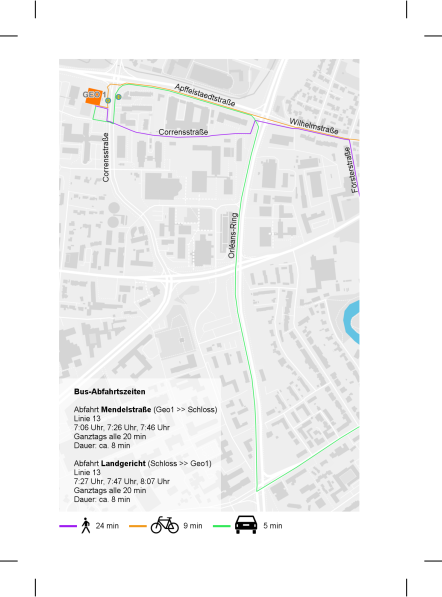
\includepdf{wegkarte-links}
\cropmarkswallpaper
%\ThisCenterWallPaper{1.0}{wegkarte-links}
%\thispagestyle{empty}

\ClearWallPaper
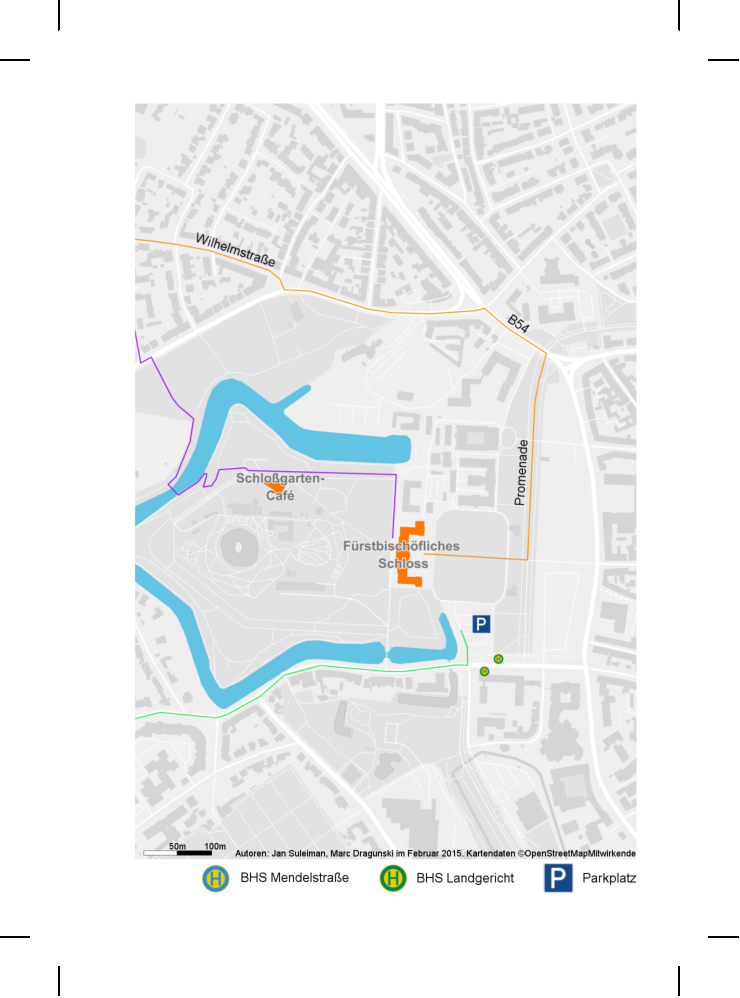
\includepdf{wegkarte-rechts}
\cropmarkswallpaper
\pagebreak

\begin{landscape}	
\ifthispageodd{\ThisCenterWallPaper{1.0}{mittwoch-ungerade}}{\ThisCenterWallPaper{1.0}{mittwoch-gerade}}
\section*{Vorträge am Mittwoch}\label{mittwoch}

\begin{center}
	\begin{longtabu}{lZ{4cm}Z{4cm}}
		& \multicolumn{1}{c}{\cellcolor{hellgruen} S\,1}
		& \multicolumn{1}{c}{\cellcolor{hellorange} Aula} \tabularnewline
		\endhead
		10:30
		\otherevent{Was ist Open-Source? Wie funktioniert das?}\coffeespace
		\talk{}{}
		\coffeespace\tabularnewline
		\rowcolor{commongray}
		12:00 & \multicolumn{2}{c}{%
			\parbox[c]{24pt}{%
				
\includegraphics[height=10pt]{cafe}%
			}
			Pause} \tabularnewline
		13:00
		\talk{}{} 
		\talk{Eröffnung}{}
		\coffeespace\tabularnewline
		13:30
		\talk{}{}
		\talk{Nicht zuschauen -- mitmachen!}{Frederik Ramm}
		\coffeespace\tabularnewline
		14:00
		\talk{}{}
		\talk{Softwarewartung für Open-Source -- ein Widerspruch?}{Till Adams}
		\coffeespace\tabularnewline
		\rowcolor{commongray}
		15:00 & \multicolumn{2}{c}{%
			\parbox[c]{24pt}{%
				
\includegraphics[height=10pt]{cafe}%
			}
			Kaffeepause} \tabularnewline
	\end{longtabu}	


	\begin{longtabu}{lZ{3cm}Z{3cm}Z{3cm}}
		& \multicolumn{1}{c}{\cellcolor{hellgruen} S\,1}
		& \multicolumn{1}{c}{\cellcolor{hellgelb} S\,2}
		& \multicolumn{1}{c}{\cellcolor{geoblau} S\,10} \tabularnewline
		\endhead
		15:30
		\talk{Welches Münster meinen sie?}{Marc Tobias Metten}
		\talk{Umsetzung der INSPIRE-Richtlinie}{Jürgen Weichand}
		\talk{Neues von QGIS 2.8}{Horst Düster}
		\coffeespace\tabularnewline
		16:00
		\talk{Offene Geodaten -- Lage von Orten im Vergleich}{Thomas Brinkhoff}
		\talk{GeoPortal.rlp}{Armin Retterath}
		\talk{QGIS-Plugins}{Pirmin Kalberer}
		\coffeespace\tabularnewline
		16:30
		\talk{OSM-Tagging in Wikidata}{Tim Alder}
		\talk{Geonetzwerk metropoleRuhr}{David Arndt}
		\talk{QGIS Print Com\-poser und Atlas-Seriendruck}{Andreas Neumann}
		\coffeespace\tabularnewline
		17:00
		\talk{Ein GeoWiki auf OSM-Basis}{Klaus Stein}
		\talk{Spatial Index von Solr}{Tim Balschmiter\vspace{0.5em}}
		\talk{QField for QGIS}{Marco Bernasocchi}
		\coffeespace\coffeespace\tabularnewline
		\rowcolor{commongray}
		17:30 &
		\multicolumn{3}{c}{%
			\textbf{Anwendertreffen/BoFs} (siehe Seite \pageref{bof-mittwoch})}
		\tabularnewline
	\end{longtabu}	
	\enlargethispage{0.5em}
\end{center}
\end{landscape}

\renewcommand{\arraystretch}{1}
% 10:30
\renewcommand{\konferenztag}{\mittwoch}
\newsmalltimeslot{10:30}
%
\abstractEins{Dominik Helle}{Was ist Open Source, wie funktioniert das?}{Die Organisation der Open Geo- und GIS-Welt. Worauf man achten sollte.}{Open Source hat viele Facetten -- und es ranken sich inzwischen ebenso viele Mythen darum. Was davon richtig ist und was nicht stellen wir in einer kurzen Einführung zusammen. Der Vortrag richtet sich an alle, die mit Open Source bisher noch wenig Kontakt hatten und die Grundlagen verstehen möchten.
	
	Open Source ist auf der einen Seite ein Entwicklungsmodell und auf der anderen ein Lizenzmodell. Zusammen bilden sie eine Kultur offener Entwicklungsgmemeinschaften, die höchst effektiv arbeiten. Diese Kultur ist um ein Vielfaches effektiver, als proprietäre Modelle es je sein können. Unter anderem sieht man das an einfachen Beispielen: Das Betriebssystem des Herstellers Apple basiert vollständig auf dem Open Source Unix FreeBSD. Es gibt halt einfach nichts besseres, und es selbst herzustellen wäre unendlich teuer. Sogar der hyper-proprietäre Hersteller Apple hat das eingesehen.
	
	Der Vortrag stellt die Geschichte der Entwicklung von Open Source vor und geht auf wichtige Grundlagen ein.
	}
%
% 13:00
\newtimeslot{13:00}
%
\abstractAula{}{Eröffnung}{}{\vspace{-2em}
	\begin{itemize}
		\setlength{\itemsep}{-2pt} % Aufzählungspunktabstand auf 0}
		\item Dominik Helle, dem FOSSGIS e.V.
		\item Prof. Dr. Edzer Pebesma, WWU Münster
		\item Olaf Knopp, WhereGroup GmbH (Goldsponsor)
	\end{itemize}
}
%
% 13:30
\newsmalltimeslot{13:30}
%
%TODO kürzen
\abstractAula{Frederik Ramm}{Nicht zuschauen -- Mitmachen!}{Zehn Arten, wie Sie OpenStreetMap voranbringen können}{OpenStreetMap lebt vom Mitmachen. Dieser Vortrag zeigt einige naheliegende und einiger weniger naheliegende Wege auf, wie auch Sie OpenStreetMap weiter voranbringen können -- als Privatperson, als Unternehmen, oder als Teil der öffentlichen Hand. 
	
	
	
	% Dass jeder bei OSM einen Account anmelden kann, ist bekannt - trotzdem schadet es nichts, das ab 
	% und zu zu wiederholen, und vor allem auf neue, einfachere Möglichkeiten der Datenerhebung hinzuweisen. 
	Viele mögen vielleicht denken, "`es ist doch schon alles da"', aber weit gefehlt -- jeder hat noch irgendwas im Kopf, was bei OSM nützlich sein kann.
	
	Das direkte Beisteuern von Daten ist aber nur einer von vielen Wegen, OSM nützlich zu sein. Auch "`indirekte"' Datenbereitstellungen -- Luftbilder, Vergleichsdaten, Straßenlisten usw. -- können dem Projekt nützen.
	
	Hacker lassen sich von den OSM-Daten zu neuer Software inspirieren und zeigen damit, was mit den freien Daten alles möglich ist. Sogar einige Unternehmen entwickeln mittlerweile Open Source Software, die in OSM eingesetzt werden kann.
	
	Privatleute und Organisationen werden Mitglied im FOSSGIS e.V. oder der OSM Foundation und stärken so die Position dieser institutionellen Stützen des OSM-Projekts. Interessierte bringen sich in die Arbeit in verschiedenen Gremien der Vereine ein - zum Beispiel bei den "Working Groups" der OSM Foundation, die immer Leute suchen.
	
	Nicht zuletzt helfen natürlich auch Geldspenden an den FOSSGIS e.V. oder die OSM Foundation, wichtige Investitionen für das Projekt zu decken.
	
	%Dieser Vortrag stellt die verschiedenen Möglichkeiten vor, OSM zu helfen - in der Hoffnung, dass für jede(n) im Publikum etwas dabei ist.
	}
%
% 14:00
\newsmalltimeslot{14:00}
%
%TODO Kürzen
\abstractAula{Till Adams}{Softwarewartung für OpenSource -- ein Widerspruch?}{}{In meinem Vortrag möchte ich ein Thema diskutieren, das sowohl die Open Source Welt, als auch die kleine, heile FOSSGIS-Welt und damit natürlich auch uns bei terrestris seit einiger Zeit umtreibt: Softwarewartung für Open Source!
	
	
	
	Wenn es darum geht, Open Source Software einzusetzen, wird dem oft das Argument 
	entgegengesetzt, das ja keiner verantwortlich sei, das es keine Betriebsgarantie 
	gibt und die Entwickler ja "morgen schon was anderes machen könnten". Ich sehe dies 
	als letzte Bastion der proprietären Hersteller im kürzlich als zu Ende erklärtem 
	Glaubenskrieg zwischen proprietärer und Open Source Software-Verfechtern.
	
%	Ich möchte in meinem Vortrag nicht diskutieren, inwieweit Architekturwechsel proprietärer 
%	Hersteller in der Vergangenheit dazu geführt haben, das Unsummen an investiertem Geld trotz 
%	sogenannter Betriebssicherheit unwiderbringlich den Rhein herabgeflossen sind. 
%	%(Stichwort ArcView GIS, Windows XP u.\,v.\,m.). 
%	Trotzdem wird solchen Anbietern eher zugetraut, das eine angebotene Softwarewartung zu Betriebs- 
%	und damit Investitionssicherheit beiträgt. 
	
	Im Vortrag steht vielmehr die Frage im Raum, ob es eine 
	Verletzung des Open Source Grundsatzes ist, wenn eine Firma, die maßgeblich hinter der 
	Entwicklung einer oder mehrerer Open Source (GIS-)Projekten steht, eine solche Wartung nach 
	proprietärem Geschäftsmodell zu einem jährlichen Fixpreis anbietet? Kann das Angebot von 
	Betriebssicherheit und auch Support dazu führen, das Open Source eher eingesetzt wird? 
	Würde ein solches Angebot überhaupt Chancen beim Kunden haben -- da sie ja anders als 
	beim proprietären Geschäftsmodell nicht obligatorisch wäre (sein kann!)? De Facto bieten 
	Firmen solche Modelle bereits an, es stellt sich die Frage, ob der Markt reif ist für 
	diese nächste "Professionalisierungsstufe"?

	}
%
% 14:30
\newsmalltimeslot{14:30}
%
% \abstractAula{Arndt Brenschede}{Lightning Talks}{}{Civic Tech in Deutschland, Intermodales ÖPNV/Rad/Fuss Routing, Hierarchische Geometrien für OSM Daten und FOSSGIS in der Hochschule}

% Für Aufzählung Abstand zwischen Aufzählungspunkten als Default in separater Variable speichern
\newlength{\itemsepdefault}
\setlength{\itemsepdefault}{\itemsep}
\abstractAula{}{Lightning Talks}{}{\vspace{-2em}
	\begin{itemize}
		\setlength{\itemsep}{-2pt} % Aufzählungspunktabstand auf 0
		\item Mila Frerichs: Civic Tech in Deutschland
		\item Arndt Brenschede:  Intermodales ÖPNV-Rad-Fuß-Routing
		\item Robert Buchholz:  Hierarchische Geometrien für OSM-Daten
		\item Arnulf Christl:  FOSSGIS in der Hochschule
	\end{itemize}
	}
%
% 15:30
\newtimeslot{15:30}
%
\abstractZwei{Jürgen Weichand}{Herausforderungen bei der Umsetzung der INSPIRE-Richtlinie}{}{Der Vortrag handelt von Datenspezifikationen, komplexen Feature-Modellen, Open Source Softwareprodukten für INSPIRE und Darstellungs- und Dounloaddiensten.
	
	Wie unterscheiden sich einfache und komplexe Feature-Modelle? Welche Lösungsansätze gibt es bei der Bereitstellung von komplexen Feature-Modellen? Mit welchen OpenSource-Softwareprodukten ist die Bereitstellung von INSPIRE-konformen Daten möglich?
	
	Weiterhin wird am Beispiel QGIS auf vorhandene Einschränkungen bei der Verwendung von Geodaten auf Grundlage von GML-Anwendungsschemata eingegangen. }
\abstractZehn{Horst Düster}{Neues von QGIS 2.8}{}{%
	Im Vortrag werden die wichtigsten neuen Features von QGIS 2.6 und der kommenden Version 2.8 vorgestellt. Es wird ein Blick auf die Entwicklung in Richtung QGIS 3 geworfen.
	
	Seit der FOSSGIS2014 in Berlin hat sich QGIS, dank der Investitionen der QGIS Anwender und der Spenden vieler Sponsoren, erheblich weiter entwickelt. Im Vortrag werden die wichtigsten neuen Features von QGIS 2.6 und der kommenden Version 2.8 vorgestellt. Ausserdem wird ein Blick auf die künftige Entwicklung in Richtung QGIS 3 geworfen.}

\abstractEins{Marc Tobias Metten}{Welches Münster meinen sie?}{Wie man Geocodern beibringt Orte mit gleichen Namen richtig zu sortieren}{%
	Wie sortiert man Orte nach Wichtigkeit, wenn sie den gleichen Namen haben? Wir schauen uns Daten zu Suchverhalten, Größe, Bevölkerungsdichte, Tagging in OpenStreetMap und Verlinkung in Wikipedia/Wikidata anhand des Nominatim Geocoders an.
	
	Der Nominatim Geocoder nutzt OpenStreetMap, minütlich aktualisiert. Die Suchergebnisse werden nach Relevanz sortiert. Einige Faktoren, wie dass Ländernamen wichtiger sind als Strassennamen sind jedem klar. Auf Mailinglisten kommt aber hin und wieder die Frage auf warum genau ein Ort wichtiger eingeschätzt wird als ein anderer.
	
%	Frankfurt gibt es zweimal, beide sind grosse Städte. Münster gibt es mehrfach. Sogar Paris, Berlin und Frankreich sobald man die ganze Welt betrachtet.
	
	Nominatim nutzt u.a. einen vorberechneten Score (numerischer Wert), der auf den Verlinkungen innerhalb Wikipedia basiert. Die erste Version sogar auf Seitenabrufen. Das hat Vor- und Nachteile (und Bugs). 
	%Leider sind selbst für Nutzer (Administratoren) von Nominatim die Algorithmen dahinter nicht transparent genug. Viele laden einfach eine selten aktualisierte Binärdatei von http://www.nominatim.org/.
	
%	Ich habe mich damit intensiver beschäftigt und plane bis zur FOSSGIS die Scripte neu schreiben und neu dokumentieren. Selbst wenn nicht wird der Vortrag ein guter Überlick werden. Ich arbeite bei http://data.opencagedata.com/index.html#about-section und wir bieten einen Geocoder u.a. auf Basis von Nominatim an http://geocoder.opencagedata.com/. Ich arbeite seit 2006 Jahren mit geocodern mit underschiedlichen kommerziellen und offenen Daten.
}

%
% 16:00
\newtimeslot{16:00}
%
%TODO könnte man noch ein klein wenig verlängern
\abstractZwei{Armin Retterath}{GeoPortal.rlp}{Ein Erfolgsmodell für den Einsatz von FOSS in der öffentlichen Verwaltung}{Dieser Vortrag illustriert anhand der Entstehungsgeschichte des rheinland-pfälzischen Geoportals, das mittlerweile auch im Saarland und in Hessen eingesetzt wird, welches immense Potential im Einsatz von FOSS-Software in der öffentlichen Verwaltung steckt. Der Vortrag diskutiert neben unerwarteten positiven Nebenwirkungen wie der verstärkten Zusammenarbeit der Verwaltungen auch Risiken und Probleme, die in der 9-jährigen Geschichte des Projekts zu bewältigen waren.}

%\abstractZehn{Pirmin Kalberer}{QGIS Plugins}{Must-Haves, Fachlösungen und Geheimtipps}{Eine grosse Stärke von QGIS ist die einfache, aber umfassende Erweiterbarkeit mittels Python Plugins. In kompakter Form wird eine Selektion aus der grossen Menge an öffentlich verfügbaren Plugins aus verschiedensten Bereichen vorgestellt.}

\abstractZehn{Pirmin Kalberer}{QGIS Plugins}{Must-Haves, Fachlösungen und Geheimtipps}{Eine grosse Stärke von QGIS ist die einfache, aber umfassende Erweiterbarkeit mittels Python Plugins. In kompakter Form wird eine Selektion aus der grossen Menge an öffentlich verfügbaren Plugins aus verschiedensten Bereichen vorgestellt. Die Auswahl geht vom bestens bekannten Open Layers Plugin und weiteren "Must-Haves" über wenig bekannte Core-Plugins wie dem Offline Editing Plugin bis zu Insidertipps wie dem Remote Debugging Plugin. Neben nützlichen Helfern werden auch umfangreiche Fachlösungen kurz vorgestellt. Es werden Anwendungsbereiche von der Datenerfassung bis zur Plugin-Entwicklung abgedeckt, aber auch Tipps gegeben, wie man selbst ein passendes Plugin findet und evaluiert.}

\abstractEins{Thomas Brinkhoff}{Offene Geodaten-Lage von Orten im Vergleich}{}{Offene Geodaten bezüglich der Lage von Orten (GeoNames Geographical Database, OSM, Wikipedia) werden vergleichend miteinander und in Bezug zu offenen amtlichen Geodaten untersucht.
	
	Untersucht wurden die Nutzbarkeit der Daten, d.\,h. Einfachheit des Zugriffs, bereitgestellte Attribute 
	und Zuordnungsmöglichkeiten zu einem gegebenen Ort,	die Vollständigkeit der Daten und die Qualität der Koordinaten.
	}
	

%
% 16:30
\newtimeslot{16:30}
%
\abstractZwei{David Arndt}{Geonetzwerk metropoleRuhr}{Die Geoinformationsplattform für das Ruhrgebiet}{Das Geonetzwerk metropoleRuhr ist eine Kooperation der Kreise und kreisfreien Städte im Ruhrgebiet mit dem Regionalverband Ruhr. Ziele sind GDI-Aufbau, Präsentation von Geodaten im eigenen Geoportal, Metadatenpflege, gegenseitige technische Unterstützung und gemeinsame Umsetzung der INSPIRE-Richtlinie.}

\abstractZehn{Andreas Neumann}{Neues vom QGIS Print Composer}{}{Der Vortrag fasst die in den letzten QGIS-Versionen eingefuehrten Verbesserungen im Print Composer 
	und im Atlas-Seriendruck zusammen. Pläne für die Entwicklung einer Reporting-Engine in einer zukünftigen QGIS-Version 
	werden vorgestellt.}


%\abstractEins{Tim Alder}{OSM-Tagging in Wikidata}{}{Der Vortrag soll beschreiben wie das OSM-Taggingschemata in Wikidata kam, wozu das Ganze zukünftig gut sein könnte und welche Unterschiede es zwischen beiden Projekten gibt. }
\abstractEins{Tim Alder}{OSM-Tagging in Wikidata}{}{%
	Wikidata ist die freie Datensammlung aus dem Wikipedia-Umfeld.
	
	Das Vorhaben das OSM-Tagging in Wikidata zu hinterlegen stellt eine Ergänzung zu dem Verlinken von OSM-Objekten mit Wikipedia-/Wikidata-Tags dar, es wird vielmehr versucht die übergeordneten OSM-Objektklassen mit Wikidata zu verbinden. Dazu wurde in Wikidata ein neues Property für das OSM-Tagging angelegt und in diesem wird das Tagging als Key oder Tag hinterlegt. 
	
	Der Vortrag wird ein paar Beispiele (Passstraße, Trafo, Tanzeinrichtung, Schuhverkäufer, Fahrradladen) aufführen, wo das Matching zwischen beiden Projekten schlecht funktioniert. Teilweise fehlen Wkipedia-Artikel. Eine 1:1-Umsetzung des OSM-Wikis kann der Links zur Wikipedia nicht sein, somit bleibt weiterhin das OSM-Wiki die verbindliche Beschreibungsseite des OSM-Taggings.
	 }

% Platz für Silber-Sponsor Geofabrik
\label{geofabrik}
\sponsorenbox{104_geofabrik}{0.53\linewidth}{-1.2em}{%
	\textbf{Silbersponsor}\\
	Die Geofabrik GmbH ist ein OpenStreetMap-Experten\-büro in Karlsruhe. 
	Seit 2007 extrahiert, filtert und verarbeitet die Geofabrik für Sie 
	freie Geodaten, erzeugt Shapefiles, Kartenbilder, Kacheln oder 
	komplette Web-Kartenanwendungen. Die Geofabrik ist spezialisiert 
	auf Dienstleistungen rund um OpenStreetMap, wie Beratung, Datenexport, 
	Server-Setup und Software-Entwicklung.}
	 
%
% 17:00
\newtimeslot{17:00}
%
%\abstractZwei{Tim Balschmiter}{Spatial Index von Solr }{Erfahrungen und Einblicke im Umgang mit Solr Spatial Index am Beispiel des Geoportal.de}{Seit der Version 4 bietet Solr Funktionen eines umfangreichen Spatial Indexes an. Am Beispiel des Geoportal.de sollen Erfahrungen und Einblicke in die Verwendung des Spatial Index mit Solr gegeben werden. }
\abstractZwei{Tim Balschmiter}{Spatial Index von Solr }{}{Seit der Version 4 bietet Solr Funktionen eines umfangreichen Spatial Indexes an. Am Beispiel des Geoportal.de sollen Erfahrungen und Einblicke in die Verwendung des Spatial Index mit Solr gegeben werden.
	
	Die GDI-DE stellt Beschreibungen und Zugangsdaten zu Geodaten von Bund, Ländern und Kommunen bereit, welche über das Geoportal.de recherchiert werden können. Über eine Volltextsuche können derzeit ca. 130000 Datensätze gefunden werden. Für einen performanten Zugriff auf die Datensätze wird die Open Source Software Solr eingesetzt. Derzeit erfolgt die Suche ausschließlich über die themenbezogenen Inhalte der Metadaten.
	}

% Was für ein Laberfassel-Abstract. Jedes Wort mehr ist heiße Marketingluft.
\abstractZehn{Marco Bernasocchi}{QField for QGIS}{}{%
QField ist die native Benutzerschnittstelle für tragbare Touchscreengeräte und bietet eine vollwertige mobile Geodaten-Verwaltungsinfrastruktur. 
Das Synchronisationtool ermöglicht einen nahtlosen Datenaustausch zwischen dem mobilen Gerät und der vorhandenen Infrastruktur.}

%\abstractEins{Klaus Stein}{Ein GeoWiki auf OSM-Basis}{}{Wikis bieten editierbare Informationen in Text und Bild, OSM geographische Objekte u.a. in Kartenform. Unser GeoWiki leistet eine enge Integration beider Konzepte, indem Textstellen direkt und interaktiv auf Geoobjekte verweisen und umgekehrt.}
\abstractEins{Klaus Stein}{Ein GeoWiki auf OSM-Basis}{}{%
	Wikis bieten editierbare Informationen in Text und Bild, OSM geographische Objekte u.a. in Kartenform. Unser GeoWiki leistet eine enge Integration beider Konzepte, indem Textstellen direkt und interaktiv auf Geoobjekte verweisen und umgekehrt.
	
	Die referenzierten und dargestellten Geoobjekte müssen dabei nicht zwingend in der OSM-Datenbank vorliegen, sondern können auch vom Nutzer im Wiki direkt angelegt werden. Zum einen senkt dies die Hemmschwelle etwas falsch zu machen, zum anderen erlaubt es die Nutzung des GeoWikis für private Daten.}

% Platz für Silber-Sponsor QGIS Enterprise
\label{qgis-enterprise}
\sponsorenbox{106_qgis_enterprise}{0.48\linewidth}{-1em}{%
	\textbf{Silbersponsor}\\
	QGIS Enterprise bietet ein kom\-plettes Wartungs- und Sup\-portpaket für den 
	Aufbau einer Geodaten-Infrastruktur (GDI). Es basiert auf den Komponenten 
	QGIS Desktop, QGIS Server, QGIS WebClient und QGIS Mobile, die getrennt vom 
	QGIS Projekt, gepflegt und gewartet werden. QGIS Enterprise ist ein Produkt 
	der Sourcepole AG und wird in Deutschland durch die Geoinformatikbüro Dassau GmbH vertrieben und betreut.}


%
% 17:30
\newtimeslot{17:30}
%
\abstractZwei{\label{bof-mittwoch}Olaf Knopp}{Mapbender Anwendertreffen}{}{}
\abstractZehn{Danilo Bretschneider}{xPlanBox Anwendertreffen}{}{}
\abstractEins{Alexey Valikov}{ows.js Entwickler-Treffen}{Entwicklung der JS-Bibliothek für OWS-Clients.}{ows.js ist ein neues OSGeo-Projekt, mit dem Ziel, eine Client-Bibliothek für die OGC Web Services in JavaScript zu implementieren.  Auf dem Entwickler-Treffen werden wir über die Anforderungen, Erfahrungen, Architektur und Entwicklung sprechen.}

% Social Event
\newpage
\ThisCenterWallPaper{1.0}{schlossgartencafe}
\thispagestyle{empty}
\section*{Social Event}
Das Social Event findet ab 19:00 Uhr im Schlossgartencafe statt. Die Teilnahme kostet 35 Euro.

\newpage
\begin{landscape}
	\renewcommand{\arraystretch}{1.4}
\ifthispageodd{\ThisCenterWallPaper{1.0}{donnerstag-ungerade}}{\ThisCenterWallPaper{1.0}{donnerstag-gerade}}
\section*{Donnerstag}\label{donnerstag}
	\begin{longtabu}{lZ{2.93cm}Z{2.93cm}Z{2.93cm}}
		& \multicolumn{1}{c}{\cellcolor{eins} S\,1}
		& \multicolumn{1}{c}{\cellcolor{zwei} S\,2}
		& \multicolumn{1}{c}{\cellcolor{zehn} S\,10} \tabularnewline
		\endhead
		09:00
		\talk{OSM und die Kunst die Welt zu ordnen}{Falk Zscheile}
		\talk{GRASS-Funktionalität in QGIS nutzen}{Otto Dassau, Sören Gebbert}
		\talk{OpenLayers 3}{Andreas Hocevar, Bart van den Eijnden, Marc Jansen}
		\coffeespace\tabularnewline
		09:30
		\talk{OSM auf Räder}{Nicole Beringer}
		\talk{Zeitreihenanalyse mit GRASS GIS}{Sören Gebbert}
		\talk{Ein Duett -- OpenLayers 3 im Zusammenspiel mit AngularJS}{Dominik Helle}
		\coffeespace\tabularnewline
		09:30
		\talk{Automatisierte OSM-Aufbereitung und Analyse von LKW-Mautstrecken in Deutschland}{Robert Klemm}
		\talk{Kreisbogen in QGIS}{Stefan Ziegler}
		\talk{GeoExt}{Christian Mayer, Marc Jansen}
		\coffeespace\tabularnewline
		\rowcolor{commongray}
		10:30 & \multicolumn{3}{c}{%
			\parbox[c]{24pt}{%
				
\includegraphics[height=10pt]{cafe}%
			}
			Kaffeepause} \tabularnewline
		11:15
		\talk{Daten aus OSM extrahieren und in QGIS weiterverarbeiten}{Claas Leiner}
		\talk{Geospatial Ruby}{Mila Frerichs}
		\talk{MapServer Pro-Tipps}{Jörg Thomsen}
		\coffeespace\tabularnewline
		11:45
		\talk{taginfo und wie es die Welt sah}{Jochen Topf}
		\talk{Jsonix -- OGC Web Services in JSON}{Alexey Valikov}
		\talk{Mapnik oder MapServer}{Oliver Tonnhofer}
		\coffeespace\tabularnewline
		12:15
		\talk{Crowd-Sourced Elevation}{Peter Barth}
		\talk{Serverseitiges JavaScript und GIS}{Christian Mayer, Marc Jansen}
		\talk{GeoServer in action}{Nils Bühner}
		\coffeespace\tabularnewline
		\rowcolor{commongray}
		12:45 & \multicolumn{3}{c}{%
			\parbox[c]{24pt}{%
				
\includegraphics[height=10pt]{restaurant}%
			}
			Mittagspause bis 13:45} \tabularnewline
		13:45
		\aulaevent{FOSSGIS-Zukunftswerkstatt}{Arnulf Christl}
		\coffeespace\tabularnewline
		14:30
		\talk{MTSatellite}{Sascha L. Teichmann}
		\talk{Erfassung von Landnutzungsveränderungen mit FOSS Image Processing Tools}{Jakob Tworek}
		\talk{Routing in der Datenbank}{Daniel Kastl}
		\coffeespace\tabularnewline
		15:00
		\talk{Straßenrennen in der Innenstadt}{Tobias Knerr}
		\talk{Automatisiertes Geodatenmanagement mit GeoKettle}{Jens Schaefermeyer}
		\talk{PostGIS Memento}{Felix Kunde}
		\coffeespace\tabularnewline
		\rowcolor{commongray}
		15:30 & \multicolumn{3}{c}{%
			\parbox[c]{24pt}{%
				
\includegraphics[height=10pt]{cafe}%
			}
			Kaffeepause} \tabularnewline
		16:00
		\talk{Prokitektura -- prozedurale realistische 3D Gebäude und Städte}{Vladimir Elistratov}
		\talk{WPS, GeoServer und SHOGun}{Till Adams}
		\talk{Docker für den GIS-Einsatz}{Bjoern Schilberg}
		\coffeespace\tabularnewline
		16:30
		\talk{Die neue WebGL-basierte Plattform für OSM-3D}{Hongchao Fan}
		\talk{Mapbender3 für den einfachen Aufbau von WebGIS Anwendungen}{Astrid Emde}
		\talk{GeoCouch}{Volker Mische}
		\coffeespace\tabularnewline
		17:00
		\otherevent{OSM Lightning Talks}
		\talk{Erfahrungen mit Sensor Web-Anwendungen}{Simon Jirka}
		\talk{Vector Tiles}{Johannes Weskamm}
		\coffeespace\tabularnewline
		\rowcolor{commongray}
		17:30
		\otherevent{PostNAS-Anwendertreffen}
		\otherevent{SHOGun BoF/Anwender- und Entwicklertreffen}\vspace{0em}
		\otherevent{deegree-Anwendertreffen}
		\coffeespace\tabularnewline
	\end{longtabu}	
\end{landscape}

\renewcommand{\konferenztag}{\donnerstag}
\newtimeslot{9:00}


% 9:00
%
\abstractEins{Falk Zscheile}{OSM und die Kunst die Welt zu ordnen}{Sprachliche und logische Aspekte 
des Taggingschemas in OpenStreetMap}{%
Anders als bei der klassischen Geodatenerfassung gibt es bei OSM keine hierarchisches gegliedertes System zur Kennzeichnung der erfassten Daten. 
Über die Frage des \glqq richtigen\grqq\  Taggings, wird sehr häufig gestritten. Oft verlaufen die Diskussionen ohne Ergebnis im Sande.

Dabei zeigt sich, dass häufig schon bei der Diskussion eines Problems aneinander vorbeigeredet wird, da der Kontext 
des Diskussionspartners nicht berücksichtigt wird. Dies zeigt sich häufig auch in einer mangelnden Auseinandersetzung mit 
Grundprinzipien der Logik. Zudem bleibt unberücksichtigt, dass sich die Tagfindung aufgrund der \glqq on the ground rule\grqq  an 
der Alltagsbedeutung von Begriffen orientiert, in den anschließenden Diskussionen aber eine feste Bedeutung im Sinne 
wissenschaftlicher Definitionen unterstellt wird.
}

\abstractZwei{Otto Dassau und Sören Gebbert}{GRASS-Funktionalität in QGIS nutzen}{}{%
	Seit 2005 ist GRASS GIS in QGIS über das GRASS Plugin integriert und stellt hunderte 
Analysemethoden über QGIS bereit -- ergänzend mittlerweile auch über das Processing und WPS Plugin. 
	
	Wir starten in diesem Vortrag einen Vergleich der drei Möglichkeiten zur Interaktion von 
GRASS und QGIS. Anhand von Beispielen stellen wir die Vor- und Nachteile dar und versuchen aufzuzeigen, 
welche Variante in welcher Situation die beste Lösung darstellt. Wann ist es sinnvoll das Processing Plugin 
zu verwenden, wann sollte man auf das bewährte GRASS Plugin setzen und welche Stärken und Schwachstellen 
bietet die Integration von GRASS Funktionalität über das WPS Plugin.
	
	Abschließend stellen wir die Aktuelle Entwicklung der Interaktion zwischen GRASS und QGIS vor und schauen in die Zukunft.}


\abstractZehn{Andreas Hocevar}{OpenLayers 3}{Stand, Neues und Zukünfiges}{%
	OpenLayers 3 wird vorgestellt, zahlreiche Beispiele zeigen die Verwendung. Unterschiede zur Vorgängerversion 
	werden aufgezeigt und auch wo und warum OpenLayers 3 anders ist. Aktuelle Entwicklungen, wie etwa das OL3-Cesium 
	Project, welches die dritte Dimension für OpenLayers zuänglich macht, werden präsentiert und ein Blick in die 
	zukünftige Entwicklung gewagt. }
%

\newtimeslot{9:30}
% 9:30
%
% Alles weitere, was im lagen Abstract steht und hier nicht auskommentiert ist, ist relativ logisch. 
% Außerdem ist der Rest des Absatzes auch mit inhaltlichen Fehlern gespickt, 
% die man niemanden lesen lassen möchte.
% Originaler Titel im Pentabarf "OSM auf Räder", nicht "OSM auf Rädern"!
%\abstractEins{Nicole Beringer}{OSM auf Räder}{}{Sind die OSM Karten soweit, um den Wettbewerb mit kommerziellen Karten im Autonavigationsbereich aufzunehmen?}
\abstractEins{Nicole Beringer}{OSM auf Räder}{}{%
	Sind die OSM-Karten soweit, um den Wettbewerb mit kommerziellen Karten im Autonavigationsbereich aufzunehmen?	
	Die Software-Unternehmen aus dem automotiven Bereich verfolgen die OSM-Entwicklung mit großer 
	Aufmerksamkeit und stehen auf der Spitze der Implementierung dieser neuen Technologie.	
}

\abstractZwei{Sören Gebbert}{Zeitreihenanalyse mit GRASS GIS}{GRASS das temporale Open Source GIS}{%
	Durch die Integration der Zeit als neue Dimension in GRASS GIS stehen nun über 45 Werkzeuge 
	zur Zeitreihenalayse bereit. 
	Eine Auswahl an Werkzeugen für die Analyse, Verarbeitung und Visualisierung von Raster- und Vektor-Zeitreihen wird vorgestellt.}

\abstractZehn{Dominik Helle}{Ein Duett -- OpenLayers 3 im Zusammenspiel mit AngularJS}{}{%
	AngularJS ist ein mächtiges Open-Source-Framework mit der clientseitige Webanwendungen nach dem MVC-Prinzip erstellt werden können. 
	OpenLayers ist wohl eine der bekanntesten Javascript-Bibliotheken um Karten im Netz nutzen zu können.
	
	Im Vortrag werden Möglichkeiten und Anregungen des Zusammenspiels dieser beiden 
	Komponenten aufgezeigt. 
	Ein erstes Aufeinandertreffen der beiden Komponenten gab es für den Autor dieses Vortrags im Rahmen eines 
	Projektes in dem eine Kartenanwendung umgesetzt wurde. Besonderes Augenmerk lag bei der Entwicklung auf der 
	schnellen und leichten anpassbar- und Wiederverwendbarkeit der Komponenten.}


\sponsorenbox{107_EB+Elektrobit}{0.43\linewidth}{-1em}{%
	\textbf{Silbersponsor}\\
	\begin{otherlanguage}{english}
	Elektrobit (EB) 
	Automotive is an international supplier of 
	embedded software solutions and services for the automotive 
	industry. With over 25 years of experience in the automotive 
	industry, EB Automotive offers flexible, innovative solutions 
	for connected car infrastructure, human machine interfaces (HMI) 
	technologies, navigation, driver assistance, ECU, and software 
	engineering services.
	\end{otherlanguage}
}
%

\newtimeslot{10:00}
% 10:00
%

\abstractEins{Robert Klemm}{Automatisierte OSM Aufbereitung und Analyse von LKW-Mautstrecken in Deutschland}{}{%
	Das beschriebene Tool erstellt mautpflichtigen Strecken anhand von Mautpunkten der Bundesanstalt für Straßenwesen (BASt). 
	Die Daten der BASt bezüglich der Strecken werden so umgewandelt, 
	dass sie in OSM abgelegt werden können. Dazu wird ein Taggingschema vorgeschlagen.
	
	Das beschriebene Tool und die damit erzeugten Mautdaten erleichtern dem Mappern die Arbeit. Für sie 
	validiert das Tool durch Routinganalyse die OSM-Daten, basierend auf dem Taggingschema mit mautbezogenen 
	Routingparametern, wie Fahrzeug-, Achs-, Gewichtsklasse und Betreiber. Es lässt sich beispielsweise die 
	schnellste und günstigste Strecke, bezogen auf die zu entrichtende Straßenmaut, ermitteln und grafisch 
	anzeigen.}

\abstractZwei{Stefan Ziegler}{Kreisbogen in QGIS}{}{Neben den gängigen Vektorelementen (Punkt, Linie, Polygon) 
	unterstützt QGIS neu Kreisbogengeometrien. Es ist jetzt möglich solche Geometrietypen 
	(ST\_CircularString, ST\_CompoundCurve, ST\_CurvePolygon etc.) aus einer Postgis-Datenbank zu lesen, anzuzeigen, zu editieren und wieder zu speichern.}

\abstractZehn{Christian Mayer und Marc Jansen}{GeoExt}{Ein ExtJS basiertes Rich-Client-WebGIS-Framework 
	in Zeiten von AngularJS und Konsorten}{%
	Der Vortrag stellt die neueste Version von GeoExt vor und zeigt auf, welches Handwerkszeug dem Entwickler 
	hier bereitsgestellt wird. Unterschiede zwischen ExtJS und anderen Bibliotheken werden benannt, dies kann 
	als Diskussionsgrundlage für die Wahl einer Bibliothek dienen. Schwerpunkt ist die Betrachtung der zukünftigen 
	Entwicklung von GeoExt.}
%

\newtimeslot{11:15}
% 11:15
%
\abstractEins{Claas Leiner}{Daten aus OSM extrahieren und in QGIS weiterverarbeiten}{Am Beispiel der Verteilung 
	von Windanlagen in Deutschland}{%
	Der Vortrag erläutert die Fragestellung am Beispiel der Verteilung von Windkraftanlagen in Deutschland. A
	ngefangen vom Import der deutschlandweiten OSM-Daten in eine PostGis-Datenbank, über die Abfrage der 
	WKA-Standorte bis hin zur Präsentation der Verteilung in einer farbigen Flächendichtekarte, die aus 
	einer interpolierten Rasteroberfläche erzeugt worden ist, welche die Anzahl der Windanlagen im Umkreis 
	von 20\,km darstellt. Dabei kamen Abfrage- und Geoverarbeitungswerkzeuge aus QGIS sowie das GRASS-Modul 
	zur Spline-Interpolation (v.surf.rst) zur Anwendung.}

\abstractZwei{Mila Frerichs}{Geospatial Ruby}{}{%
	Der Talk gibt einen Überblick darüber, was mit Ruby im Geo Bereich möglich ist. Viele große 
	erfolgreiche Webprojekte sind mit Ruby und dem dazugehörigen Webframework Rails umgesetzt worden. 
	
	 Der Fokus dieses Vortrags liegt auf drei wichtigen Bibliotheken terraformer.rb, rgeo und SimpleTile.}

\abstractZehn{Jörg Thomsen}{MapServer Pro-Tipps}{Das \emph{Do what I want} Know How für den UMN MapServer}{%
	MapServer ist bekannt für seine Zuverlässigkeit, Performance und Stabilität. Gerne wird 
	aber auch über die Konfiguration mit den Mapfiles gestöhnt. Dabei bietet gerade diese Art der 
	Konfiguration Möglichkeiten, die tief in der Dokumentation versteckt sind und die bei kniffligen 
	Augaben wirklich hilfreich sein können. Die meisten Anwender kennen nur die Basis-Konfigurationen, 
	aber wer weiß schon dass es einen eingebauten OpenLayers-Client gibt, der es ermögicht nur mit einem 
	Mapfile eine interakive Karte zu veröffentlichen, wie man Linien mit Pfeilspitzen versieht, Geometrien 
	glättet oder den Zugriff auf MapServer-WMS direkt im Mapfile auf bestimmte IP-Adressen beschränken kann?
	
	Weitere Themen des Vortrags sind PHP-Fassaden, JOINs mit Datei basierten Datenquellen, ColorRanges, Cluster von Punktobjekten, Geomtransform und IP-Zugriffsbeschränkungen.}
%

\newtimeslot{11:45}
% 11:45
%
\abstractEins{Jochen Topf}{Taginfo und wie es die Welt sah}{}{%
	Das OpenStreetMap-Projekt organisiert seine Daten über ein offenes Taggingschema. 
	Jeder kann neue Objekte und Tags erfinden und in der OSM-Datenbank speichern. 
	Dieser Vortrag stellt den Web-Dienst Taginfo vor, der Informationen zu Tags aus 
	verschiedenen Quellen darstellt und Mappern so hilft, die Übersicht zu behalten. 
	Der Vortrag geht sowohl auf die alltägliche Nutzung als auch auf weniger bekannte Seiten des Dienstes ein.}

\abstractZwei{Alexey Valikov}{Jsonix: OGC Web Services in JSON}{}{%
	JSON hat wahrscheinlich XML schon längst als Lingua franca ersetzt. 
	Es ist viel leichtgewichtiger und einfacher zu verwenden als XML, vor 
	allem in den JavaScript-basierten Web-Apps.
	
	Das Web GIS Umfeld wird von JavaScript-Bibliotheken wie OpenLayers und Leaflet dominiert. 
	Für die gehört JSON sowieso zur Muttersprache. Aber die OGC-Standards sind fast alle XML-basiert 
	und durch XML Schemata spezifiziert.
	
	Jsonix ist eine Open-Source Bibliothek für die XML<->JS Konvertierung, die genau das möglich macht. 
	Mit Jsonix kann man ein XML Schema nehmen und daraus eine Mapping-Datei erzeugen.
	Dieser Vortrag gibt eine Überblick von Jsonix und zeigt es Live in WMS, WFS, CSW sowie OL3 WPS Client Demos vor.}

\abstractZehn{Oliver Tonnhofer}{Mapnik oder MapServer}{Wer macht die schönsten Kartenß}{%
	Mit Mapnik und MapServer stehen zwei OpenSource Kartenrenderer zur Verfügung, die in Geschwindigkeit, 
	Funktionsumfang und Bildqualität kaum Wünsche übrig lassen. Aber welche Software nehme ich für mein Projekt?
	
	Der Vortrag geht auf die kleinen und großen Unterschiede zwischen Mapnik und MapServer ein. Für welche 
	Einsatzzwecke ist MapServer besser geeignet? Was kann Mapnik besonders gut? Wie können die Renderer in 
	Anwendungen und Server integriert werden? Gibt es überhaupt nennenswerte Unterschiede?}
%

\newtimeslot{12:15}
% 12:15
%
\abstractEins{Peter Barth}{Crowd-Sourced Elevation}{DIY DEM}{%	
	Digitale Höhenmodelle können für eine Vielzahl von Anwendungen im OpenStreetMap-Umfeld verwendet werden. 
	In Renderstilen werden sie z.\,B. für Schummerungen oder Höhenlinien verwendet. 
	Aber auch bei Routinganwendungen gibt es verschiedenste Gründe, das Geländemodell mit zu beachten: 
	Fahrradfahrer, Rollstuhlfahrer aber auch Energiesparen bei Elektromobilität.
	
	Mit SRTM steht ein genaues Höhenmodell mit nahezu globaler Abdeckung gemeinfrei zur Verfügung und 
	erst kürzlich wurde auch die Version mit einer Auflösung von einer Bogensekunde freigegeben. Aber reicht das?
	
	Nach einem Überblick über das Thema Höhenmodelle und die verschiedenen Datenquellen wird anhand von Experimenten und 
	deren Auswertung gezeigt, wie man mit einem handelsüblichen Smartphone selbst ein Höhenmodell erstellen 
	kann. Eignen sich die Methoden für Crowdsourcing und wie gut ist das Ergebnis verglichen mit SRTM?}

\abstractZwei{Christian Mayer}{Serverseitiges JavaScript und GIS}{Mit Node.js und npm die Welt beherrschen}{Der 
	Vortrag gibt eine allgemeine Einführung in die Node.js-Welt und zeigt wie mit Node.js geo-relevante Probleme, 
	wie das Einlesen von GIS-Datenformaten sowie die Verarbeitung von Geodaten möglich wird. Ebenso wird eine 
	Übersicht von nützlichen Node.js-Modulen aus dem GIS-Bereich sowie Beispielanwendungen vorgestellt.}

\abstractZehn{Daniel Koch}{GeoServer in action}{Fortgeschrittene Möglichkeiten beim Einsatz des GeoServers}{%
	Der GeoServer ist ein weithin bekannter und mächtiger OpenSource Kartenserver. Sofern man die Umgebung 
	eingerichtet hat, ist sowohl die Installation als auch die Konfiguration von ersten WMS- und WFS-Layern sehr einfach. 
	In diesem Vortrag wird auf die typischen Anforderungen eines \glqq GeoServers in action\grqq\ eingegangen. Der Vortrag fokussiert 
	sich also weniger auf die \glqq Out-of-the-box\grqq{}-Verwendung des GeoServers, sondern beleuchtet vielmehr fortgeschrittene 
	Möglichkeiten beim Einsatz dieser Software.
	
	Themen des Vortrags sind das Kompilieren, die Verwendung der REST-Schnittstelle, Extensions, Performance-Tuning, GeoWebCache-Einsatz, Troubleshooting und Stolperfallen.}
%

\newtimeslot{13:45}
% 13:45
%
\abstractAula{Arnulf Christl}{FOSSGIS-Zukunftswerkstatt}{Menschen begeistern im FOSSGIS-Verein mitzuwirken
	}{%
	Wer steckt hinter dem FOSSGIS e.V.? Um diese Frage zu beantworten veranstaltet der FOSSGIS e.V eine Zukunftswerkstatt. 
	Erfahren Sie mehr über Ziele, Strukturen und Menschen im Verein. 
	Lassen Sie sich begeistern von der Idee gemeinsam etwas zu bewegen. }
\vspace{-1em}
\sponsorenbox{101_52n}{0.38\linewidth}{-1em}{%
	\textbf{Silbersponsor}\\
	52$^\circ$\,North ist ein offenes in\-ternationales Forschungs- und Ent\-wick\-lungsnetzwerk im Bereich der Geoinformatik. 
	Partner aus Forschung, Industrie und Verwaltung  arbeiten aktiv an  Innovationsthemen, die aus den 
	Forschungslabors in die breite praktische Anwendung gebracht werden. Die 52$^\circ$\,North GmbH dient dem 
	Netzwerk als Geschäfts- und Koordinierungsstelle sowie als Service-Center. Kernaufgabe ist die 
	Entwicklung neuer Konzepte und Technologien in der Geoinformatik, insbesondere in den Bereichen 
	Sensor Web und Web basiertes Geoprocessing. Darüber hinaus bietet 52$^\circ$\,North auf Basis seiner 
	Erfahrungen und Technologien Dienstleistungen in den Bereichen Consulting und Software-Entwicklung an.}
\newpage\noindent%\sponsorenbox{105_terrestris}{0.45\linewidth}{-1em}{%
%	terrestris bietet Dienstleistungen und Produkte mit Open Source Software an und 
%	ist dabei insbesondere auf Geodateninfrastrukturen, webbasierte Informationssysteme und WebMapping-Anwendungen fokussiert, 
%	die neben 2D auch 3D Daten enthalten und auch für mobile Endgeräte optimiert sind.
%	
%	Wir orientieren uns dabei an den Anforderungen unserer Kunden und realisieren auf 
%	den jeweiligen Bedarf zugeschnittene Lösungen.
%	Neben der Anwendungsentwicklung können unsere Kunden Support und Schulungen für 
%	verschiedene Open Source Softwaretools, z. B. PostgreSQL/PostGIS, UMN Mapserver, 
%	GeoServer, SHOGun, OpenLayers, GeoExt, ExtJS und QGIS, erhalten.
%	
%	National und international gut vernetzt bieten wir zusammen mit unseren Partnerfirmen
%	Wartung und Support zu Open Source Produkten/Projekten wie SHOGun, GeoServer oder OpenLayers an.
%	Diese Rahmenbedingungen erlauben uns unvoreingenommen Lösungen zu entwickeln und 
%	anzubieten, die tatsächlich alle Anforderungen unserer Kunden zufrieden stellen.
%}
%
\vfill
\setlength{\fboxsep}{4.5pt}
\noindent\fcolorbox{gray}{white}{\parbox{\fboxwidth}{%
	\begin{wrapfigure}{r}{0.3\textwidth}
		\vspace{-1em}
		\centering 
		
\includegraphics[width=\linewidth]{105_terrestris}
		\vspace{-1em}
	\end{wrapfigure}	
	\textbf{Silbersponsor}\\	
	\noindent terrestris bietet Dienstleistungen und Produkte mit Open Source Software an und 
	ist dabei insbesondere auf Geodateninfrastrukturen, webbasierte Informationssysteme und WebMapping-Anwendungen fokussiert, 
	die neben 2D auch 3D Daten enthalten und auch für mobile Endgeräte optimiert sind.
	
	Wir orientieren uns dabei an den Anforderungen unserer Kunden und realisieren auf 
	den jeweiligen Bedarf zugeschnittene Lösungen.
	Neben der Anwendungsentwicklung können unsere Kunden Support und Schulungen für 
	verschiedene Open Source Softwaretools, z. B. PostgreSQL/PostGIS, UMN Mapserver, 
	GeoServer, SHOGun, OpenLayers, GeoExt, ExtJS und QGIS, erhalten.
	
	National und international gut vernetzt bieten wir zusammen mit unseren Partnerfirmen
	Wartung und Support zu Open Source Produkten/Projekten wie SHOGun, GeoServer oder OpenLayers an.
	Diese Rahmenbedingungen erlauben uns unvoreingenommen Lösungen zu entwickeln und 
	anzubieten, die tatsächlich alle Anforderungen unserer Kunden zufrieden stellen.
	}
}
\setlength{\fboxsep}{3pt}
\vfill

\newtimeslot{14:30}
% 14:30
% Der Untertitel ist ewig lang und der Inhalt steht auch so im Abstract.
\abstractEins{Sascha L. Teichmann}{MTSatellite}{Echtzeit Webmapping für Minetest-Welten oder Spiel-Spass mit GIS}{%
	Der Vortrag stellt die Freie Software MTSatellite vor, ein Live-Webmapping System für das Open World/Sandbox-Spiel Minetest 
	(eine Open-Source-Alternative zu Minecraft). 
	Der Vortrag führt das System vor und gibt eine teils vertiefende Übersicht über die eingesetzen Technologien sowohl aus GIS- 
	als auch aus Sicht eines passionierten Minetest-Spielers.}

\abstractZwei{Jakob Tworek}{Erfassung von Landnutzungsveränderungen mit FOSS Image Processing Tools}%
{%Change Detection mit QGIS - Landnutzungs- und -bedeckungsveränderungen erfassen
	}{%
	In diesem Vortrag wird eine Masterarbeit am Geographischen Institut der Universität Bonn vorgestellt. Im Rahmen dieser Masterarbeit 
	wurde zwei Change-Detection-Verfahren mit freier Bildverarbeitungssoftware angewandt und evaluiert.
	Zu den verwendeten Programmen zählen das Semi-Automatic Classification Plugin und Image Processing Tools der Orfeo Toolbox 
	und SAGA im Rahmen des Processing Framework von QGIS.
	}

\abstractZehn{Daniel Kastl}{Routing in der Datenbank}{Kürzeste-Wege-Berechnung und mehr mit pgRouting}{Die pgRouting-Erweiterung 
	ermöglicht es, auf Daten in einer PostgreSQL-Datenbank eine kürzeste-Wege-Suche und andere 
	netzorientierte Algorithmen anzuwenden. Neben den etablierten Funktionen sind für die nahe 
	Zukunft eine Reihe neuer Algorithmen zur Tourenplanung zu erwarten. Dieser Vortrag stellt 
	die verschiedenen Algorithmen vor und geht darauf ein, wie die Struktur der Netzdaten die Leistung des Systems beeinflussen kann.}

% Platz für Silber-Sponsor Camptocamp
\sponsorenbox{102_C2C-logo-baseline-RGB_PSE}{0.4\linewidth}{-1em}{%
	\textbf{Silbersponsor}\\
	Camptocamp ist ein innovatives Unternehmen im Bereich der Integration 
	von Software zum Aus\-werten von Geodaten, zur kompletten Verwaltung von 
	Unternehmen (ERP) und zur Verwaltung von Daten-Infrastrukturen.}

\newtimeslot{15:00}
% 15:00
%
\abstractEins{Tobias Knerr}{Straßenrennen in der Innenstadt}{SuperTuxKart-Strecken bauen mit OSM2World}{%
	Der Gründer des Open-Source-Projekts OSM2World erzählt von einer weiteren spannenden Anwendungsmöglichkeit des 3D-Renderers -- die 
	Erstellung von Rennstrecken für das freie Computerspiel SuperTuxKart.
	
	Der Vortrag beschreibt die Vorgehensweise, um die OSM-Daten einer Stadt in eine Rennstrecke zu 
	verwandeln. Voraussetzung ist eine ausreichend gute Abdeckung der jeweiligen Region mit 3D-Attributen in OpenStreetMap.
	
	Aus diesen Daten wird mit dem 3D-Renderer OSM2World ein realitätsnahes 3D-Modell erstellt, das optional 
	auch mit einem Geländemodell ergänzt werden kann. Mit dem 3D-Modelling-Tool Blender noch einige 
	Verbesserungen vorgenommen und der gewünschte Streckenverlauf eingezeichnet. Ein Blender-Plugin 
	erlaubt schließlich den Export einer fertigen Strecke für SuperTuxKart.	
}

\abstractZwei{Jens Schaefermeyer}{Automatisiertes Geodatenmanagement mit  GeoKettle}{}{%
	Dieser Vortrag stellt verschiedene Einsatzmöglichkeiten der freien ETL-Software GeoKettle vor. 
	GeoKettle ist die Open-Source-Alternative zur verbreiteten Software FME und kann nicht nur Geodatenformate konvertieren, 
	sondern beispielsweise auch Objekte verteilen und zusammenfassen, redundante Daten 
	finden oder Prozesse in einer grafischen Oberfläche modellieren.}

\abstractZehn{Felix Kunde}{PostGIS Memento}{Versionierung von PostGIS-Datenbanken}{Memento. Gibt es nicht 
	einen Film, der so heißt? Jemand, der kein Gedächtnis hat und sich alle Ereignisse aufschreibt? 
	Zumindest geht es bei pgMemento darum. pgMemento zeichnet alle Veränderungen in einer 
	PostgreSQL Datenbank auf und erlaubt die Wiederherstellung beliebiger frühere Zeitstände.}
%

\newtimeslot{16:00}
% 16:00
%
\abstractEins{Vladimir Elistratov}{Prokitektura -- prozedurale realistische 3D Gebäude und Städte}{}{%
	Prokitektura is ein prozedurales und iteratives Verfahren für Schaffung architektonischer 3D Modelle. 
	
	Ein Satz kleiner Funktionen auf Python wird verwendet um 3D Gebäude zu generieren.
	Eine solche Funktion nennt man Regel. Jede nachfolgende Regel verfeinert das Modell 
	und ergänzt es mit zusätzlichen Details. Zur Zeit ist Prokitektura als ein Add-on für 
	Open Source 3D Plattform Blender realisiert.}

\abstractZwei{Till Adams}{WPS, GeoServer und SHOGun}{}{Der Vortrag stellt die Erweiterung des SHOgun 
	Frameworks als WPS-CLient dar. Als WPS Server kommt der GeoServer-WPS zum Einsatz. Der Vortrag 
	wird zum einen kurz die Mechanismen des WPS erläutern, die Einbindung in das SHOGun Framework an 
	praktischen Beispielen zeigen und am Ende die Möglichkeiten, die sich daraus für ein WebGIS ergeben vorstellen. }

\abstractZehn{Bjoern Schilberg}{Docker für den GIS-Einsatz}{}{Mit der leichtgewichtige Virtualisierungs-Software 
	Docker schnell und einfach Anwendungs-Container für Ihre GIS-Fachanwendung erstellen. Haben die 
	GIS-Admins demnächst wieder mehr Zeit für ungleich spannendere Aufgaben als die Installation von Fachanwendungen?}

% Platz für Silbersponsor Omniscale
% wir verzichten auf Absätze, da diese meist eh nur einen Satz lang sind 
% und die Sätze noch nicht ewig lang sind
\sponsorenbox{103_omniscale}{0.38\linewidth}{-1em}{%
	\textbf{Silbersponsor}\\
	Omniscale ist Spezialist für die Bereitstellung von schnellen und attraktiven Karten auf Ba\-sis von OpenStreetMap und amtlichen Daten.
	Unter maps.omniscale.com bietet Omniscale kostengünstige Kartendienste für 
	Desktop-GIS und Online-Anwendungen an. Zusätzlich entwickelt Omniscale für 
	Wirtschaft, Industrie und Behörden individuelle Kartendienste. Verlässlich, 
	schnell und attraktiv.
	Neben den Kartendiensten entwickelt Omniscale auch moderne Kartenanwendungen 
	auf Basis von Open-Source-Software. Omniscale ist zudem Initiator und Hauptentwickler 
	der Open-Source-Projekte MapProxy und Imposm.
}

\newtimeslot{16:30}
% 16:30
%
\abstractEins{Hongchao Fan}{Die neue WebGL-basierte Plattform für OSM-3D}{}{%
	In diesem Vortrag wird die technische Archtektur, das Funktiondesign und die 
	Implementierung der neue WebGL-basierte Plattform von OSM-3D präsentiert. 
	Es werden interaktive Visualisierungen der 3D Stadtmodelle und 3D Geländemodelle 
	demonstriert. Das neue Interface für interaktive Erfassungen von Dach- und 
	Fassadenstrukturen wird vorgestellt und mit Beispielen demonstriert. 
	Diskussion von Vorschlägen zur Verbesserungen der neuen Plattform. }

\abstractZwei{Astrid Emde}{Mapbender\,3 für den einfachen Aufbau von WebGIS Anwendungen}{So einfach ist 
	der Aufbau von WebGIS Anwendungen mit Mapbender3}{Mapbender3 ist eine Software zur einfachen 
	Erstellung von WebGIS Anwendungen. Der Vortrag geht vor allem auf die neuen Komponenten in 
	Mapbender3 ein und stellt diese vor. Anpassung an das eigne Layout, Suchen in eignen Daten und Rechteverwaltung werden thematisiert.}

% Der kurze Abstract ist auch gut.
%\abstractZehn{Volker Mische}{GeoCouch}{Ein multidimensionaler Index für Couchbase}{%
%	GeoCouch ist ein multidimensionaler Index für Couchbase, einer verteilten dokumentenorientierten Datenbank. 
%	Dieser Vortrag wird eine kurze Einführung in Couchbase, die räumliche Abfragen ermöglicht, 
%	und die Datenmodellierung geben und dann in eine Live-Demonstration übergehen. }
\abstractZehn{Volker Mische}{GeoCouch}{Ein multidimensionaler Index für Couchbase}{%
	Couchbase ist eine verteilte dokumentenorientierten Datenbank und gehört damit 
	zur Kategorie der NoSQL Datenbanken. Das bedeutet, dass das Datenmodell nicht 
	relational ist, also ein gewisses Umdenken bei der Strukturierung der Daten nötig ist. 
	GeoCouch ist in Couchbase integriert und ermöglicht räumliche Abfragen. Diese sind nicht 
	auf zwei Dimensionen begrenzt, sondern können durch weitere Attribute erweitert werden. 
	So ist es möglich Faktoren, wie Zeit, Ausmaß oder Kategorien einzubeziehen. Eine beispielhafte 
	multidimensionale Datenbankabfrage wären alle Einwohner eines bestimmten Gebiets, die unter 30 
	Jahre alt sind und in einer Mietwohnung mit weniger als 50m$^2$ wohnen. Dieser Vortrag wird eine 
	kurze Einführung in Couchbase und die Datenmodellerung geben und dann in eine 
	Live-Demonstration übergehen.}
% Platz für Bronzesponsor Büro Dassau
\sponsorenbox{209_gbd-consult}{0.34\linewidth}{-1.3em}{%
	\textbf{Bronzesponsor}\\
Die Geoinformatikbüro Dassau GmbH bietet Lösungen für die Umsetzung 
von GIS Projekten auf Open Source Basis und ist spezialisiert auf die 
Software GRASS und QGIS.
}

%

\newtimeslot{17:00}
% 17:00
\abstractEins{Christoph Hormann (Moderation)}{OSM Lightning Talks}{}{}\vspace{-2em}
\abstractZwei{Simon Jirka}{Erfahrungen mit Sensor Web-An\-wendungen für mobile Geräte und Desktop-Anwendungen}{}{%
	Dieser Vortrag stellt einen freien, auf JavaScript basierenden Sensor Web-Client vor, 
	der auf allen Arten von Endgeräten von Mobiltelefonen bis hin zu Desktop-PCs einsetzbar ist. 
	Er geht auf die Entwicklung des Clients und auf seine Nutzung als eigenständige Software und 
	als Basis eigener Projekte ein.}

\abstractZehn{Johannes Weskamm}{Vector Tiles}{Performante Übertragung von umfangreichen Vektordaten}{%
	Es werden die Vor- und Nachteile von Vectortiling und der Vektordaten-Prozessierung im Client allgemein beleuchtet. 
	Als praktischer Anwendungsfall wird das Prinzip der Vectortiles anhand des Software-Stacks 
	TileStache, OpenLayers3 und PostGIS auf Basis von OSM-Daten vorgestellt.}
%

\newsmalltimeslot{17:30}
% 17:30
\vspace{-2em}
\abstractEins{Olaf Knopp}{PostNAS Anwendertreffen}{}{%
	PostNAS ist ein Projekt zum Import von ALKIS Daten über OGR. Es werden aktuelle Entwicklungen des Projekt vor\-gestellt.}
\abstractZwei{\label{bof-donnerstag}Till Adams}{SHOGun BoF/Anwender- und Entwicklertreffen}{}{Es wird der aktuelle 
	Entwicklungsstand von SHOgun, neue Ideen und auch neue Entwicklungen, die seit der FOSSGIS 2014 dazu gekommen sind, vor\-gestellt.}
\abstractZehn{Danilo Bretschneider}{deegree Anwendertreffen}{}{deegree ist ein Open-Source Java-Framework für 
	die Verwaltung und Darstellung OGC-konformer Geoinformationssysteme.}
%

\newsmalltimeslot{19:30}
% 19:00
%
%\abstractSenatssaal{}{Vollversammlung FOSSGIS e.V.}{}{}
	\thispagestyle{scrheadings} 
	\setlength\tabcolsep{0pt}
	\noindent\fcolorbox{white}{dezentrot}{\parbox{\titleboxwidth}{%
		\noindent\begin{tabu}{X[5L]r}
			& \talktime
			\tabularnewline
			\noindent\bfseries \normalsize \sectfont Vollversammlung FOSSGIS e.V.
			&
			Senatssaal
			\tabularnewline
		\end{tabu}%
	}}
	%
	\setpagebackground%
	\vspace{0.5em}% Abstand zum nächsten Talk, auch wenn es keinen Abstract gibt
	\setlength\tabcolsep{6pt} % Spaltenpadding wieder auf Default setzen
	
\sponsorenbox{207_intevation}{0.4\linewidth}{-1.3em}{%
	\textbf{Bronzesponsor}\\
Die Intevation GmbH ist ein produkt- und hersteller\-un\-ab\-hängiger IT-Dienstleister, 
welcher konsequent auf freie Software setzt. Mit unserer  bald fünfzehnjährigen praktischen 
Erfahrung haben wir eine Vielzahl von spannenden  Projekten mit den Themen Geographische 
Informationssysteme und  Webanwendungen, Netzwerk-Sicherheit, Email-Servern, 
Email-Kryptographie,  Groupware, Datenbanken, Sozialinformatik, Software-Paketierung  
und -Qualitätssicherung realisiert.
}
\vfill
\sponsorenbox{208_Kuestenschmiede}{0.34\linewidth}{-1.3em}{%
	\textbf{Bronzesponsor}\\
Wir entwickeln Webanwendungen, speziell zur Darstellung von Geoinformationen in 
Kombination mit Content Management Systemen (CMS). Dabei setzen wir auf verschiedene 
Open-Source-Projekte wie die OpenStreetMap,  OpenLayers, die Overpass API und auf das 
CMS Contao. Auf der FOSSGIS 2015 präsentieren wir als Aussteller unseren GIS-Baukasten 
con4gis, der es ermöglicht, auf einfache Weise komplexe, interaktive Geoinformationssysteme 
auf Webseiten bereitzustellen.
}

\newpage
\vfill
\noindent
\sponsorenbox{206_norBIT}{0.31\linewidth}{-1em}{%
	\textbf{Bronzesponsor}\\
Als Softwarehaus für GIS-Kom\-plett\-lösungen entwickelt die norBIT GmbH seit über 25 Jahren mit norGIS 
modular aufgebaute Fachschalen für Anwendungen im Bereich von Tiefbau, Ver- und Entsorgung, die mit 
verschiedenen Grafikplattformen, wie QGIS, AutoCAD und BricsCAD betrieben werden (ggf. auch gemischt).
Seit über 8 Jahren beteiligt sich die norBIT GmbH an der Weiterentwicklung des QGIS und nutzt die 
Software zur Erfüllung verschiedenster Kundenanforderungen von Auskunftslösungen bis zu GIS-Arbeitsplätze.
Mit dem norGIS-ALKIS-Import und dem ALKIS-Plugin für QGIS hat die norBIT GmbH eine Open-Source-Lösung 
für die Verarbeitung und Visualisierung von ALKIS-Daten in QGIS und UMN Mapserver geschaffen.
}

\begin{landscape}
	\renewcommand{\arraystretch}{1.4}
\ifthispageodd{\ThisCenterWallPaper{1.0}{freitag-ungerade}}{\ThisCenterWallPaper{1.0}{freitag-gerade}}
\section*{Vorträge am Freitag}
\label{freitag}
	\begin{longtabu}{lZ{2.93cm}Z{2.93cm}Z{2.93cm}}
		& \multicolumn{1}{c}{\cellcolor{hellgruen} S\,1}
		& \multicolumn{1}{c}{\cellcolor{hellgelb} S\,2}
		& \multicolumn{1}{c}{\cellcolor{geoblau} S\,10} \tabularnewline
		\endhead
		08:45
		\talk{Indoor Routing in Gebäuden des ÖPNV auf Basis von OSM}{Thomas Jakubicka}
		\talk{Projekt Umweltzone}{Tobias Preuß}
		\talk{Öffentliche Projekte und Open Source}{Sven Böhme}
		\coffeespace\tabularnewline
		09:15
		\talk{Neues zu BRouter}{Arndt Brenschede}
		\talk{Verkehrs\-mittel\-bezogenen Er\-reich\-barkeit}{Marc Beiling}
		\talk{Das audiovisuelle Erbe der OSGeo-Projekte}{Peter Löwe}
		\coffeespace\tabularnewline
		09:45
		\otherevent{OSM Lightning Talks II}
		\talk{Linked Data basierter Explorer}{Friedrich Müller}
		\talk{Wie wird man ein FOSSGIS-Open Source Projekt?}{Oliver Tonnhofer, Till Adams}
		\coffeespace\tabularnewline
		\rowcolor{commongray}
		10:15 & \multicolumn{3}{c}{%
			\parbox[c]{24pt}{%
				
\includegraphics[height=10pt]{cafe}%
			}
			Kaffeepause} \tabularnewline
		11:00
		\talk{Schatzsuche in OpenStreetMap}{Roland Olbricht}
		\talk{Location-based Task Management}{Daniel Kastl}
		\talk{3D GIS Stack aus OpenSource Komponenten}{Felix Kunde}
		\coffeespace\tabularnewline
		11:30
		\talk{FlatMatch -- Online-Woh"-nungs"-su"-che mit OSM-Daten}{Robert Buchholz}\coffeespace
		\talk{MapFish Print V3: Printing maps like a boss}{Tobias Sauerwein}
		\talk{Cesium - der 3D-Globus im Web}{Elisabeth Leu}
		\coffeespace\tabularnewline
		\rowcolor{commongray}
		12:00 & \multicolumn{3}{c}{%
			\parbox[c]{24pt}{%
				
\includegraphics[height=10pt]{cafe}%
			}
			Kaffeepause} \tabularnewline
		\rowcolor{hellorange}
		12:30
		\aulaevent{Abschlussveranstaltung}{}
		\tabularnewline
		\rowcolor{hellorange}
		13:30 & \multicolumn{3}{c}{%
			\parbox[c]{24pt}{%
				
\includegraphics[height=10pt]{bar}%
			}
			\textbf{Sektempfang} (Aula)} \tabularnewline
		\coffeespace\tabularnewline
	\end{longtabu}
	\ThisCenterWallPaper{1.0}{freitag-ungerade-gedreht}	
\end{landscape}
\renewcommand{\arraystretch}{1}
\renewcommand{\konferenztag}{\freitag}
\newtimeslot{8:45}

\abstractEins{Thomas Jakubicka}{Indoor Routing in Gebäuden des öffentlichen Verkehrs auf Basis von OpenStreetMap Daten}{}{%
	In unserem Vortrag möchten wir unser Konzept der Indoor-Navigation vorstellen und Erfahrungen und \glqq Best Practices\grqq\  
	präsentieren die wir bei der Indoor Erfassung von Gebäuden des öffentlichen Verkehrs gemacht haben. }

\abstractZwei{Tobias Preuß}{Projekt Umweltzone}{zwischen Open Data und OpenStreetMap}{%
	In diesem Vortrag wird das Projekt \glqq Umweltzone\grqq\ vorgestellt. Dabei handelt es sich 
	um eine kostenlose Open-Source-Anwendung für Android-Geräte, mit der sich Benutzer 
	über die Lage der Umweltzonen verschiedener deutscher Städte informieren können. 
	Die Herausforderung bestand in der Recherche, Beschaffung, Digitalisierung bzw. 
	Umwandlung und Integration der Geoinformation zu den Umweltzonen. 
	
	Im Vortrag wird auch über den Verlauf und Erfolg der Wochenaufgabe \emph{Umweltzonen} im August 2014 in der deutschen OSM-Community berichtet. }

\abstractZehn{Sven Böhme}{Öffentliche Projekte und Open Source}{Open Source Software in der öffentlichen Verwaltung am Beispiel der GDI-DE Testsuite}{%
	Anhand der GDI-DE Testsuite wird dargestellt, wie die GDI-DE die Strukturen von Open Source Projekten, 
	wie sie u.a. durch die OSGeo beschrieben werden, in Ihren Komponenten verwendet. Betriebsstelle GDI-DE 
	im Bundesamt für Kartographie und Geodäsie (BKG) wurde als Schnittstelle zwischen der fachlichen und der 
	technischen Umsetzung geschaffen. Der Vortrag bietet einen Einblick in die tägliche Arbeit der Betriebsstelle. 
	Die Ziele sowie die Hürden im täglichen Betrieb werden vorgestellt.}
\sponsorenbox{205_metaspatial}{0.38\linewidth}{-1em}{%
	\textbf{Bronzesponsor}\\
Haben Sie die perfekte Komplettlösung? Ist was offen geblieben? Wir 
beraten seit über 15 Jahren Unternehmen und Behörden bei Fragen 
rund um die Geodatenverarbeitung mit Open-Source, Open-Standards und Open-Data. 
Nutzen Sie unsere Kompetenzen und lernen Sie wie agiles 
Projektmanagement optimal beim Aufbau von nachhaltigen, wartbaren 
und skalierbaren Architekturen erfolgreich zum Einsatz kommt.
}
%
% 9:15
\newtimeslot{9:15}

\abstractEins{Arndt Brenschede}{Neues zu BRouter}{Mehr als nur Outdoor-Navigation}{%
	Dieser Vortrag stellt einige der Neuerungen aus dem letzten Jahr beim Projekt BRouter vor, 
	die selbst die regelmässigen Nutzer noch kaum kennen.
	Beispiele sind steigungsabhängige Weg-Präferenzen, schnellere Neuberechnungen und die Integration der 30m-SRTM Höhendaten.
	
	Die wichtigste Neuerung aber ist ein neues, flexibleres internes Datenmodell. 
	Dadurch werden sowohl Spezialanwendungen im Wegenetz möglich, etwa im Hinblick auf Barrierefreiheit, 
	Einsatzfahrzeuge oder Schwerlastverkehr, aber auch Anwendungen in ganz anderen Netzen wie dem Schienen, Fluss- oder Stromnetz.}

% zusätzliches vspace wegen mehrzeiliger Titel nötig
\abstractZwei{Marc Beiling}{Verkehrsmittelbezogene Erreichbarkeitsvisualisierung der Ruhr-Universität Bochum\vspace{0.3em}}{%
	Eine beispielhafte Mappinganwendung im Mobilitätskontext}{%
	Der Vortrag behandelt die Anwendung Verkehrsmittelbezogene Erreichbarkeitsvisualisierung für 
	Studierende der Ruhr-Universität Bochum, die als beispielhafte Umsetzung zu verstehen ist. 
	Die Herausforderungen beim Routing mit OSM-Daten werden aufgezeigt und Neulingen im 
	OSM/FOSS-Bereich wird ein Einblick in netzwerkbasierte Berechnungen/Visualiserungen 
	und dafür zu verwendende Komponenten ermöglicht.}

\abstractZehn{Peter Löwe}{Das audiovisuelle Erbe der OSGeo-Projekte }{Referenzfall GRASS GIS - und Star Trek}{%
	Dieser Vortrag diskutiert die Problematik der Archivierung aller Aspekte von Open Source-Projekten und 
	stellt das AV-Portal der Technischen Informationsbibliothek (TIB) vor. Das Portal ist eine zukunftssichere 
	Alternative zum häufig praktizierten eher flüchtigen Datenaustausch über Plattformen wie Youtube oder 
	Slideshare und kann nicht nur Metadaten eines Videos indexieren, sondern auch die gesprochene Sprache, 
	Texteinblendungen oder Bildinformationen.
	Durch die Verbindung eines DOI mit einem Media Fragment Identifier wird die sekundengenaue Zitierfähigkeit der Materialien gewährleistet. 
	
	Der Nutzen wird am Beispiel der erfolgreichen digitalen Erschließung des GRASS GIS Videos des U.S. 
	Army Corps of Engineers Research Laboratory (CERL) aus dem Jahr 1987 demonstriert.}

%
% 9:45
\newtimeslot{9:45}
%
\abstractEins{Christoph Hormann (Moderation)}{OSM Lightning Talks II}{}{}\vspace{-2em}

\abstractZwei{Friedrich Müller}{Linked Data basierter Explorer}{%
	Ein Assistenzsystem zur Erforschung von Umweltdaten für krebsrelevante Ursache-Wirkungs-Beziehungen im raum-zeitlichen Kontext}{%
	Aktuell ist eine Vielzahl krebsbezogener Informationen als Open-Data verfügbar. Allerdings sind diese Datensätze oft 
	nicht aggregiert, in unterschiedlichen Formate oder teilweise nur unter erhöhtem Arbeitsaufwand zugänglich. Die hier 
	präsentierte Webanwendung vereinfacht, auf Basis von Linked Data und weiteren semantischen Technologien, die Erreichbarkeit 
	krebsrelevanter Informationen. Neben der Möglichkeit sich über die krebsbezogenen Ursache-Wirkungs-Beziehungen zu informieren, 
	ist der Hauptnutzen der Applikation die ermöglichte Erforschung von Umweltdatenim Zusammenhang 
	mit epidemiologischen Datensätzen u.\,a. per Geovisualisierungen für die Beispielregion Westfalen-Lippe.
	
	Der Workflow basiert komplett auf freier Software/Daten, (z.\,B. Protegé, Apache Jena, R, OSM und Leaflet). 
	Produkte des Projektes sind neben dem Quellcode zur Wiederverwendung auf Github zugänglich.}

% kann man noch länger machen, wenn man keine Werbung hat
\abstractZehn{Oliver Tonnhofer und Till Adams}{Der schwere Werdegang zu einem FOSSGIS-Open Source Projekt}{}{%
	OpenSource machen ist einfach. Ein bisschen Code geschrieben, einen schicken Lizenz-Header oben drüber gepastet 
	und ab damit auf Git oder eine andere hippe Plattform. Aber damit ist es dann meistens doch nicht getan. 
	Der Vortrag beschreibt warum.}
\sponsorenbox{203_CS_Gis}{0.34\linewidth}{-1em}{%
	\textbf{Bronzesponsor}\\
CSGIS verfügt über langjährige Erfahrung bei der Durchführung von GIS-Projekten 
mit Open Source Technologie in den Bereichen Desktop GIS und WebGIS und engagiert 
sich bei der Entwicklung diverser Open Source Projekte. Wir wünschen Ihnen eine 
erfolgreiche FOSSGIS 2015 Konferenz! 
}
%
% 11:00
\newtimeslot{11:00}
% Variante 1 ist auch gut
%\abstractEins{Roland Olbricht}{Schatzsuche in OpenStreetMap}{}{%
%	Mit der Overpass API lassen sich auch ungewöhnliche Daten in OpenStreetMap finden -- und bewundern, 
%	ihnen nachspüren oder sie korrigieren. Neben einer Präsentation der Ergebnisse des Vergleiches von 
%	Bonn und Münster werden dabei auch ausführlich die verwendeten Overpass-API-Abfragen vorgestellt, 
%	sodass jeder die Abfragen leicht für seine Stadt wiederholen oder inhaltlich auf seine Bedürfnisse anpassen kann.}
\abstractEins{Roland Olbricht}{Schatzsuche in OpenStreetMap}{}{%
	Mit der Overpass API lassen sich auch ungewöhnliche Daten in OpenStreetMap finden -- und bewundern, 
	ihnen nachspüren oder sie korrigieren. 
	
	Wir untersuchen zwei Großstädte, Bonn und Münster, mit verschiedenen Ansätzen auf ungewöhnliche Daten. 
	Was bleibt, wenn man alle Objekte weglässt, die sich anhand ihrer Tags einer klaren Kategorie zuordnen lassen? 
	Wo fehlen wahrscheinlich noch Briefkästen? Welche Brücken haben keine Höhenangabe? 
	Wo steht in den Tags eines Elements vermutlich Spam? Welche Restaurants (und sonstige Points of Interest) sind verdächtig alt?
	
	Neben einer Präsentation der Ergebnisse werden dabei auch ausführlich die verwendeten Overpass-API-Abfragen vorgestellt, 
	sodass jeder die Abfragen leicht für seine Stadt wiederholen oder inhaltlich auf seine Bedürfnisse anpassen kann.}
\abstractZwei{Daniel Kastl}{Location-based Task Management}{Standortbezogene Aufgabenverwaltung für mobile Arbeitsplätze}{%
	FOSS4G Software kann bei vielerlei Aufgaben mit Raumbezug helfen, Arbeitsabläufe zu verbessern und zu optimieren, und 
	die Mitarbeiter bei Ihrer täglichen Arbeit zu entlasten. Dieser Vortrag stellt ein Konzept für Location-based Task Management vor.
	
	Mit der Optimierung von Arbeitsabläufen und Tourenplanung im Hinterkopf, und auf Grundlage verfügbarer Open-Source-Software 
	und offenen Standards haben wir begonnen, eine Task-Management-Software zu entwickeln. In dieser Präsentation 
	werden Sie Details zu unserem Konzept zu erfahren, und wie dies dazu beitragen kann, Dienstleistungen vor Ort 
	zu erleichtern, die Servicequalität zu verbessern und die Effizienz zu steigern.}

\abstractZehn{Felix Kunde}{3D GIS Stack aus OpenSource Komponenten}{}{%
	In den letzten Jahren hat die dritte Dimension auch Einzug in den gängigen FOSSGIS Lösungen (PostGIS, QGIS, OpenLayers etc.) 
	gehalten, so dass mittlerweile ein kompletter 3D-GIS-Stack aus OpenSource Lösungen realisiert werden kann. 
	Das wichtigste Ziel der hier vorgestellten Projekte ist die Interaktion mit 3D-Webkarten. Der Anwender soll 
	in der Lage sein, mit den 3D-Modellen über das Web arbeiten zu können und sie nicht nur zu betrachten.}

%
% 11:30
\newtimeslot{11:30}
\abstractEins{Robert Buchholz}{FlatMatch -- Online-Wohnungssuche mit OSM-Daten}{Können wir tausende deutsche Vermieter zu OSM-Mitwirkenden machen?}{%
	FlatMatch ist eine Web-Anwendung, um Mietwohnungen direkt im Webbrowser virtuell zu besichtigen und so eine geeignete neue Wohnung zu finden. 
	Hierzu wird die Wohnung \emph{und}, basierend auf OSM-3D-Gebäuden und TileMaps die Aussicht aus der Wohnung interaktiv dreidimensional dargestellt.
	
	Dies vereinfacht für Mieter die Wohnungssuche und erlaubt Vermietern, den Personalaufwand für Besichtigungen zu reduzieren, 
	und ihre Wohnungen auch auf Basis deren Umfelds zu vermarkten.
	Die Mitarbeit kommerzieller Nutzer an OSM hängt jedoch allein davon ab, ob sie dadurch einen 
	wirtschaftlichen Mehrwert erhalten. FlatMatch könnte zehntausende kleine und mittlere Unternehmen in Deutschland 
	diesen Mehrwert bieten.}

% zusätzliches vspace wegen langem Titel
\abstractZwei{Tobias Sauerwein}{MapFish Print V3 -- Printing maps like a boss\vspace{0.3em}}{}{%
	Das Projekt MapFish Print besteht aus einer Bibliothek und einer Web-Anwendung zum Druck von Reports mit Karten, 
	wobei eine Vielfalt von Quellen unterstützt wird, z.\,B. WMS, WMTS, OpenStreetMap-Kacheln, WFS oder GeoJSON.
	Dieser Vortrag stellt die neue Version von MapFish Print vor und spricht Themen an wie die neuen Features und 
	deren Nutzung, die Erstellung von Templates mit dem Report-Designer von JasperReports, Upgrade von der 
	vorherigen Version, Skalierbarkeit und Erweiterung durch eigene Module.}

\abstractZehn{Elisabeth Leu}{Cesium -- der 3D-Globus im Web}{}{%
	Cesium ist eine JavaScript-Bibliothek, mit der 3D-Globen für das Web erstellt werden können. 
	Cesium nutzt WebGL und unterstützt ausserdem OGC-Standards wie WMS oder WMTS.
	
	Im Vortrag werden folgende Fragen beantwortet: Was kann Cesium? Performante mehrdimensionale Visualisierung im Web -- was steckt dahinter? 
	Wo wird überall Cesium eingesetzt? Ausserdem wird die Kombination von Openlayers3 mit Cesium vorgestellt 
	und ein Ausblick über die künftige Entwicklung gegeben.}
%
% 12:30
\newtimeslot{12:30}
%
\abstractAula{Marco Lechner}{Abschlußveranstaltung}{}{%
Die Abschlussveranstaltung der FOSSGIS-Konferenz 2015 blickt auf die gelaufene Konferenz 
und auf die nächste. Wir dürfen alle gespannt sein. In diesem Rahmen findet auch die Verlosung 
statt, an der alle teilnehmen, die den Teilnehmerfeedbackbogen ausgefüllt haben.}
%
% 13:30
\newsmalltimeslot{13:30}
\vspace{-1em}
\abstractAula{Katja Haferkorn}{Sektempfang}{}{}
\vspace{-2.5em}
\sponsorenbox{204_mapwebbing}{0.38\linewidth}{-1em}{%
	\textbf{Bronzesponsor}\\
Die Firma Mapwebbing, ge\-gründet 2008 von Lars Lingner Dipl.-Inf.(FH), 
mit Sitz in Berlin im Büro 2.0 ist spezialisiert auf die Planung und 
Erstellung von individuellen Kartenlösungen. Kernkompetenz ist die 
Entwicklung und Umsetzung maßgeschneiderter Konzepte zur Verarbeitung 
von Geodaten, über Kartenrendering bis hin zur Frontendentwicklung für 
den Kunden. Seit neu\-stem stellt die Firma Mapwebbing Dienstleistungen 
zum Erstellen von Kartenmaterial für den professionellen Druck zur 
Verfügung. Lars Lingner setzt bei allen Projekten auf freie und 
offene Software und Daten (z.\,B. OpenStreetMap).
}
\enlargethispage{1em}

\vfill
\setlength{\fboxsep}{4.5pt}
\noindent\fcolorbox{gray}{white}{\parbox{\fboxwidth}{
\begin{wrapfigure}[5]{r}{0.4\textwidth}
	\begin{center}
		\vspace{-1.7em}
		
\includegraphics[width=\linewidth]{202_DBG}
%		\vspace{-2em}
	\end{center}
\end{wrapfigure}
\textbf{Bronzesponsor}\\
Seit 1991 realisiert die \mbox{d.b.g.} Datenbankgesellschaft mbH innovative Softwarelösungen 
für das Management von Freiflächen und für die Durchführung von Verkehrssicherheitskontrollen. 
Das Portfolio reicht dabei von Systemen zur Verwaltung von Bäumen, Spielgeräten und Freiflächen 
über Anwendungen zur Betriebssteuerung und Planung bis hin zu Dienstleistungen in den 
Bereichen Luftbildinterpretation und Baumkontrolle. Speziell im Bereich GIS werden 
Schulungen und Beratungen durchgeführt, Schnittstellen für freie Open-Source- und 
kommerzielle Systeme entwickelt, Geodaten veredelt und über ein eigenes WebGIS zur Verfügung gestellt. 
}
}
\setlength{\fboxsep}{3pt}
\vfill
\setlength{\fboxsep}{4.5pt}
\noindent\fcolorbox{gray}{white}{\parbox{\fboxwidth}{
		\begin{wrapfigure}[3]{r}{0.44\textwidth}
			\begin{center}
				\vspace{-1.3em}
				
\includegraphics[width=\linewidth]{201_MapMedia}
				%		\vspace{-2em}
			\end{center}
		\end{wrapfigure}
		\textbf{Bronzesponsor}\\
		Wir erschließen das räumliche Potenzial Ihrer Daten! Die MapMedia GmbH 
		ist Ihr Dienstleister für digitale Kartographie und raumbezogene Informationssysteme. 
		Bei der Durchführung von Projekten setzen wir bevorzugt und erfolgreich freie Software (Open-Source) ein.
	}
}
\setlength{\fboxsep}{3pt}
\vfill

\ClearWallPaper

\includepdf{sponsorenseite}
\cropmarkswallpaper
\setlength{\fboxsep}{4.5pt}
\noindent\fcolorbox{gray}{white}{\parbox{\fboxwidth}{
		\begin{wrapfigure}[6]{r}{0.47\textwidth}
			\begin{center}
				\vspace{-1.3em}
				
\includegraphics[width=\linewidth]{210_beMasterGIS_final}
				%		\vspace{-2em}
			\end{center}
		\end{wrapfigure}
		\textbf{Bronzesponsor}\\
		Mit dem online-ge\-stütz\-tem Fernstudiengang zum Mas\-ter Geo\-in\-for\-mations\-sys\-teme (Master of Engineering) 
		an der Hochschule Anhalt am Campus Dessau -- haben Fachanwender von Geoinformationssystemen (GIS) 
		die Chance Ihr Fachwissen entsprechend zu erweitern. Zielgruppe sind Anwender von 
		Geoinformationssystemen, die in der kommunalen Verwaltung, 
		im Planungsbereich, im Umwelt- und Naturschutz, in der 
		Versorgungswirtschaft, im Marketing und anderen Bereichen arbeiten oder die Verbindung mit 
		GIS mit ihrem persönlichen Arbeitsumfeld planen. Das berufsbegleitende fünfsemestrige Fernstudium 
		entspricht in Qualität, Umfang und Wertigkeit einem Direktstudium, es  kommt mit wenigen 
		Präsenzphasen aus, bis zu zwei Semester sind für die Anfertigung der Masterthesis vorgesehen.
			}
		}
		\setlength{\fboxsep}{3pt}
\newpage

\ClearWallPaper

\includepdf{sponsorenseite}
\cropmarkswallpaper
\newpage
\section*{Impressum}
\label{impressum}
\vspace{-0.5em}

%\ThisCenterWallPaper{1.0}{crop-marks}

\RaggedRight
Die FOSSGIS 2015 wird gemeinsam vom FOSSGIS e.V. und der Universität Münster 
organisiert.

\vspace{0.5em}
	
\includegraphics[width=0.43\linewidth]{FOSSGIS}
	\hfill
	
\includegraphics[width=0.43\linewidth]{logo-rgb-ifgi-text-de.pdf}

\vspace{0.5em}
\noindent Verantwortlich für den Inhalt:\\
FOSSGIS e.V.\\
Theodor-Echtermeyer-Straße 15\\
14469 Potsdam

\vspace{0.5em}
\noindent Diese Programmheft wurde von Michael Reichert, Katja Haferkorn, 
Jan Suleiman, Marc Dragunski und Frederik Ramm unter Verwendung von \LaTeX\ und 
anderer freier Software zusammengestellt.\\
{\small Quellcode: github.com/Nakaner/fossgis-2015-booklet}

\vspace{0.5em}

{\small\noindent Geodaten: 
\includegraphics[height=7pt]{copyright}~Open\-Street\-Map-Mitwirkende, osm.org/copyright\\
Karte auf Seite \pageref{inhaltsverzeichnis} und \pageref{karte}: Jan Suleiman, Marc Dragunski\\
Rückseite: Deutscher Mapnik-Stil, CC-BY-SA~2.0, bearbeitet und gerendert durch Frederik Ramm\\
Icons in den Tabellen: SJJB Management, CC-0\\
Gebäudeskizze: WWU-Grewer
}


\vspace{1em}
\noindent \begin{minipage}[htbp]{0.2\textwidth}
\noindent
\includegraphics[width=\linewidth]{cc-by-sa-pdf}
\end{minipage}
\hfill
\begin{minipage}[hbtp]{0.74\textwidth}\RaggedRight
Alle Inhalte dieses Programmhefts unterliegen, sofern nicht anders angegeben, 
der Creative Commons Namensnennung Weitergabe unter gleichen Bedingungen 3.0.
\end{minipage}



\begin{landscape}
	\label{gebaeudeplan}
	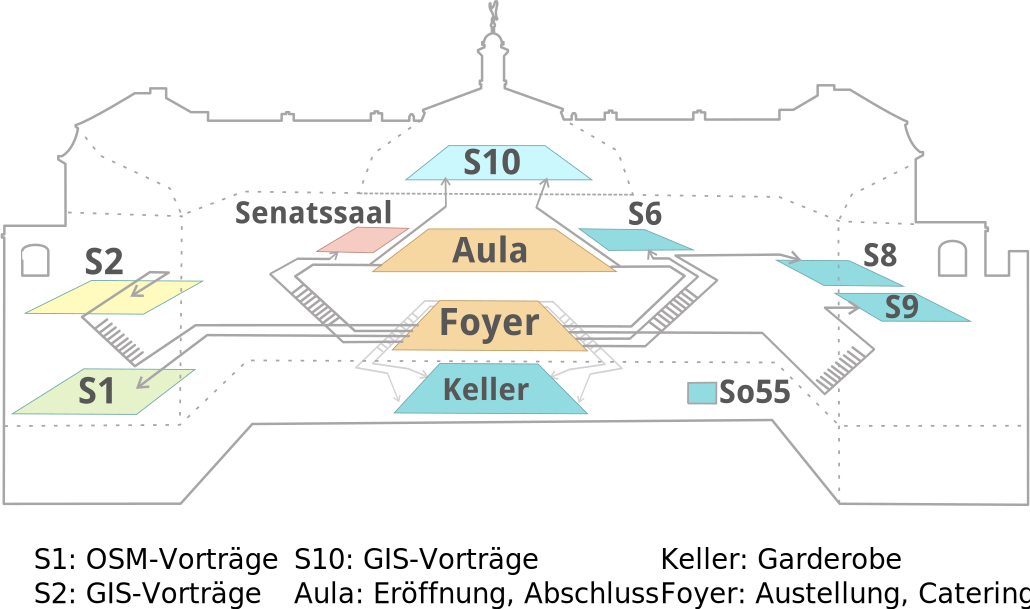
\includegraphics[width=\linewidth]{gebaeudeplan}
	
	{\small Bildquelle: WWU-Grewer, bearbeitet}
\end{landscape}


\label{karte}
%
\ClearWallPaper
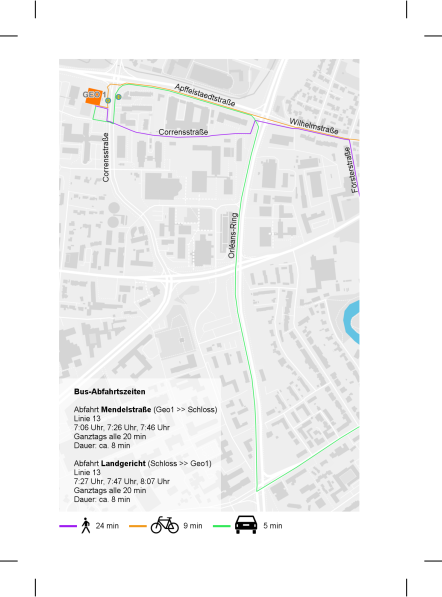
\includepdf{wegkarte-links}
\cropmarkswallpaper
%\ThisCenterWallPaper{1.0}{wegkarte-links}
%\thispagestyle{empty}

\ClearWallPaper
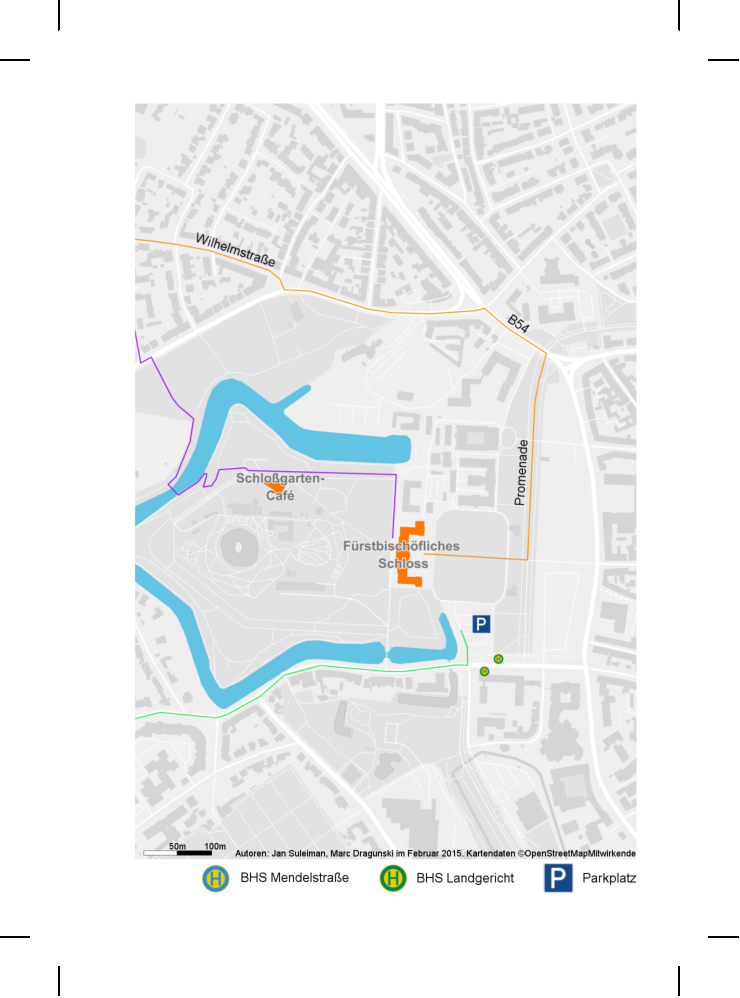
\includepdf{wegkarte-rechts}
\cropmarkswallpaper
\pagebreak
\newpage\begin{center}

\includegraphics[width=0.4\linewidth]{001_Wheregroup}
\hfill

\includegraphics[width=0.4\linewidth]{301_oreilly}

\noindent
\includegraphics[width=0.4\linewidth]{101_52n}
\hfill

\includegraphics[width=0.4\linewidth]{102_C2C-logo-baseline-RGB_PSE}

\noindent
\includegraphics[width=0.4\linewidth]{103_omniscale}
\hfill

\includegraphics[width=0.4\linewidth]{104_geofabrik}

\noindent
\includegraphics[width=0.3\linewidth]{105_terrestris}
\hfill

\includegraphics[width=0.4\linewidth]{106_qgis_enterprise}


\includegraphics[width=0.4\linewidth]{107_EB+Elektrobit}
\hfill

\noindent
\includegraphics[width=0.3\linewidth]{201_MapMedia}
\hfill

\includegraphics[width=0.3\linewidth]{202_DBG}
\hfill

\includegraphics[width=0.3\linewidth]{203_CS_Gis}

\noindent
\includegraphics[width=0.2\linewidth]{208_Kuestenschmiede}
\hfill

\includegraphics[width=0.4\linewidth]{205_metaspatial}
\hfill
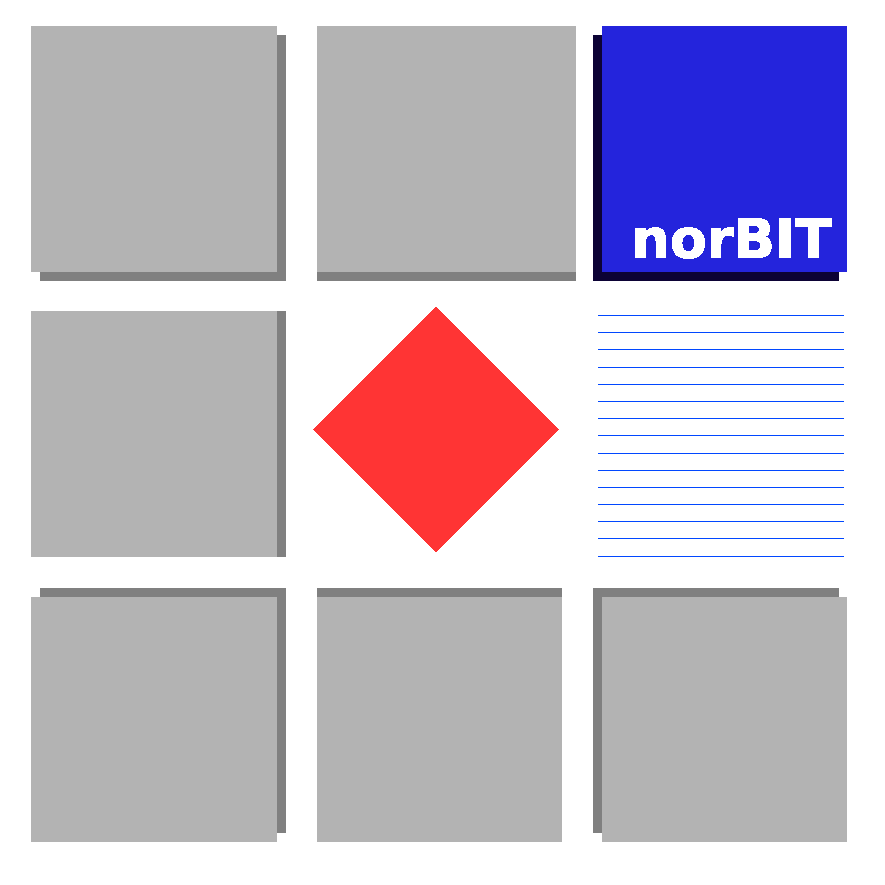
\includegraphics[width=0.15\linewidth]{206_norBIT}

\noindent
\includegraphics[width=0.3\linewidth]{204_mapwebbing}
\hfill

\includegraphics[width=0.2\linewidth]{207_intevation}
\hfill

\includegraphics[width=0.2\linewidth]{209_gbd-consult}

\noindent
\includegraphics[width=0.2\linewidth]{210_beMasterGIS_final}






\end{center}


\end{document}
